\documentclass[11pt, a4paper]{article}

\usepackage[a4paper, margin=2.5cm]{geometry}
\usepackage{fontspec}
\usepackage[english, bidi=basic, provide=*]{babel}
\babelprovide[import, onchar=ids fonts]{english}
\babelfont{rm}{Noto Sans}

\usepackage{amsmath}
\usepackage{booktabs}
\usepackage{array}
\usepackage{tabularx}
\usepackage{longtable}
\usepackage{xcolor}
\usepackage{graphicx}
\usepackage[font=small]{caption}
\usepackage{enumitem}
\usepackage{xurl}
\usepackage{seqsplit}
\urlstyle{tt}
\makeatletter\def\UrlBreaks{\do\/\do\_\do\.\do\-}\def\UrlBigBreaks{}\makeatother\Urlmuskip=0mu\relax
\usepackage[hidelinks]{hyperref}

\definecolor{navy}{HTML}{1B365D}
\definecolor{slate}{HTML}{4A5568}
\definecolor{rulegray}{HTML}{CBD5E0}
\definecolor{panelbg}{HTML}{F7FAFC}

\hypersetup{
    colorlinks=true,
    linkcolor=navy,
    urlcolor=navy,
    citecolor=navy,
    pdftitle={Mitochondrial tRNA-Tyr C33 in four fish lineages occurs without a genome-wide signature of UAA-to-tyrosine reassignment},
    pdfauthor={Thomas Biondi}
}

\linespread{1.08}
\emergencystretch=4em
\setlength{\parskip}{0.45em}
\setlength{\parindent}{0pt}

\begin{document}

% --- TITLE BLOCK ---
{\noindent\small\color{slate}\textbf{PREPRINT} \quad|\quad Evolutionary Biology / Genomics \quad|\quad Pre-registered Study (v3)}
\vspace{0.35em}
{\color{rulegray}\hrule height 0.8pt}
\vspace{1.0em}

{\LARGE\bfseries\color{navy}\raggedright
Mitochondrial tRNA-Tyr C33 in four fish lineages occurs without a genome-wide signature of UAA-to-tyrosine reassignment\par}

\vspace{0.9em}
{\large\textbf{Thomas Biondi}$^{*}$}

\vspace{0.3em}
{\small\color{slate}
Independent Researcher\\
$^{*}$Corresponding author: \href{mailto:tcb.dna@gmail.com}{tcb.dna@gmail.com}
}

\vspace{0.6em}
{\footnotesize\color{slate}
\textbf{Pre-registration:} \texttt{PREREG.md}, SHA-256 \texttt{\seqsplit{e23bc13f37ca48647b86cdc6b3d70abc5f7e0b69c71968de05e7b32285b4fa0c}} (locked 2026-11-23, commit \texttt{5aa5774}).\\
\textbf{Code \& Data:} \url{https://github.com/tcbDNA/tbiondi-genomics/tree/main/metazoan-mito-uaa-tyr} (commit \texttt{35bf5df}).\\
\textbf{Evidence labels:} \texttt{[C]} pre-registered confirmatory; \texttt{[E]} pre-planned exploratory; \texttt{[S]} the \texttt{PREREG} weak tier, reported for sensitivity only; \texttt{[P]} post-hoc.
}

\vspace{0.8em}
{\color{rulegray}\hrule height 0.5pt}
\vspace{0.8em}

% --- ABSTRACT ---
\section*{Abstract}
Lin et al.\ (2026) reported that, among bivalves, a U33C change in the anticodon loop of mitochondrial tRNA-Tyr(GUA) occurs only in lineages that read UAA as tyrosine, never under canonical code 5; Zhao et al.\ (2026) linked reassignment to parallel changes in this tRNA and release factor mtRF1a. We tested how far this exclusivity generalises in a pre-registered screen of 32,982 mitogenomes. Of 28,583 UAA=Stop genomes with a resolved tRNA-Tyr, 17 were non-U33 screen positives (0.059\%); 9 of 12 vertebrate C33 calls are elopomorphs \texttt{[P]}. Six fish from four lineages (code 2) have independent same-species C33 support and lack a genome-wide UAA=Tyr signature \texttt{[P]}: none has an internal UAA at 71--72 conserved tyrosine sites, and 11 or 12 of 13 genes end in UAA, encoded or completed by polyadenylation (RNA confirms 7 and 6 genes in two species). C33 in two bonefishes was tabulated without comment (Satoh et al.\ 2016). A contig search that recovers a hidden U33 copy in \textit{Globodera ellingtonae} found no second tRNA-Tyr in the six, down to about half mitochondrial depth. No C33 genome was confirmed among 16,902 code-5 UAA=Stop genomes, including 489 bivalves. C33 alone does not mark UAA=Tyr in code 2, which is compatible with tRNA--mtRF1a co-evolution; mtRF1a S216 occurred in 0 of 47 UAA=Stop species tested. \textit{Rotylenchulus reniformis}, whose genus NCBI already assigns code 14 (UAA=Tyr), has strong sequence evidence for it but failed a locked stem rule; the zero-new-clade null is weak, because the molecular gates pass 14 of 20 known positives.

\vspace{0.5em}
\noindent\textbf{Keywords:} mitochondrial genetic code, codon reassignment, tRNA-Tyr, mtRF1a, comparative mitogenomics, pre-registration

% --- INTRODUCTION ---
\section{Introduction}
Mitochondrial genetic codes have departed from the standard nuclear code repeatedly across Metazoa. One such departure is the reassignment of the termination codon UAA to tyrosine (Tyr). Independent UAA=Tyr reassignments have been documented in pterobranch hemichordates (\textit{Cephalodiscus}, NCBI translation table 33; Li et al.\ 2019), plant-parasitic nematodes of the genus \textit{Radopholus} (Jacob et al.\ 2009), tanaidacean crustaceans (\textit{Pseudotanais}; Jakiel et al.\ 2025; Matsushima et al.\ 2026), and several clades of pteriomorphian bivalves (Anomiidae, Placunidae, and Plicatulidae; Lin et al.\ 2026; Zhao et al.\ 2026). It remains a question how a single-codon stop signal comes to be decoded as sense without catastrophic readthrough, and whether specific structural substitutions in the decoding apparatus act as general drivers across phyla.

Two recent studies proposed specific molecular correlates of mitochondrial UAA=Tyr reassignment. Zhao et al.\ (2026) reported parallel U33C substitutions in the anticodon loop of mitochondrial tRNA-Tyr(GUA) together with a parallel T191S substitution in mitochondrial translation release factor 1a (mtRF1a) across several UAA=Tyr lineages. U33C is predicted to disrupt recognition by tRNA-guanine transglycosylase (TGT) and abolish queuosine modification of the wobble base G34; T191S corresponds to T216S in human \texttt{NP\_061914.3}. They noted exceptions in \textit{Radopholus similis} and \textit{Pseudotanais}. Independently, Lin et al.\ (2026) analysed bivalve mitogenomes and reported a consistent U-to-C substitution in the tRNA-Tyr anticodon loop, which they call ``U36C'' in their alignment numbering and which we infer is canonical position 33. They state that it occurs exclusively in UAA=Tyr lineages and is absent from all species that retain the canonical invertebrate mitochondrial code 5. That statement was made for bivalves and for code 5; here we ask whether it holds outside that domain. Earlier, Li et al.\ (2019) also stated that starfish, which retain UAA=Stop under echinoderm code 9, carry a C at position 33 of tRNA-Tyr. That appears to contradict Zhao et al., who depict U33 in \textit{Asterias rubens}.

C33 has been tabulated in fish before. Satoh et al.\ (2016) recorded the base at every tRNA position in 250 fish mitogenomes. Their Table S7 gives C at position 33 of tRNA-Tyr (position 39 in their numbering) in 2 of 250 and T in 248, without naming the two species or discussing them. Their list includes two bonefish records that carry C33 in our calls, \texttt{AP002973} (filed as \textit{Albula glossodonta}) and \textit{Pterothrissus gissu} (\texttt{AB051197}, the source of \texttt{NC\_005796}), so these are the two.

Our question is how far Lin et al.'s code-5 exclusivity generalises. Does C33 also mark UAA=Tyr in other lineages and under other translation tables, or can it occur where UAA still reads as a stop? The answer also bears on Zhao et al.'s model. If tRNA and release factor co-evolve, a C33 tRNA-Tyr beside an unchanged mtRF1a (T216) is an allowed state, so C33 genomes with ordinary coding sequences would limit C33 as a stand-alone marker without arguing against co-evolution. Testing this across animals requires searching broad public mitogenome archives while guarding against thresholds tuned after the fact, misannotated assemblies, nuclear mitochondrial DNA segments (NUMTs), heteroplasmy, and hidden second tRNA loci on multipartite genomes.

Here we report a pre-registered, metazoan-wide screen of 32,982 eligible public mitogenomes, paired with targeted mtRF1a profiling in reassigned clades, flagged candidates, and phylogenetic sisters. Before running any caller on non-control genomes, we calibrated the UAA and tRNA-Tyr callers on a control panel of 360 genomes (334 of them are among the 32,982; the other 26 are not) and locked all classification thresholds, structural locus-identity audits, and named statistical tests in a hashed pre-registration document (\texttt{PREREG.md}). After the confirmatory sweep and two cold reviews (round 1 by the same model family, round 2 blind and by a different model), we ran targeted post-hoc stress tests on every key candidate. They include exact read-power bounds, competitive depth mapping to circular mtDNA, similarity-independent searches of high-copy contigs for hidden second tRNA copies, audits of specimen metadata, a per-gene audit of terminal stops and poly(A) ends in the six best-supported fish, and a pre-specified local assembly test of \textit{Rotylenchulus reniformis}. Throughout, outcomes are labelled explicitly as confirmatory \texttt{[C]}, exploratory \texttt{[E]}, \texttt{PREREG} weak-tier \texttt{[S]} (sensitivity only), or post-hoc \texttt{[P]}.

% --- RESULTS ---
\section{Results}

\subsection{Pre-registered screen design, calibration, and detection limits}
A total of 32,982 metazoan mitogenomes met the pre-registered eligibility criteria. They come from RefSeq release 238, NCBI organelle assemblies, and eligible INSDC-only records; 98 records were excluded for length, ambiguity, or by pre-registration, and 8,189 \texttt{UNVERIFIED}-flagged and 5,635 incomplete INSDC-only entries were withheld. The set comprises 32,623 confirmatory non-panel genomes (31,564 NCBI taxa), 358 records of panel species (334 panel genomes and 24 other records of the same species), and one named extra, \texttt{AP002973.1}, retained only for a targeted Albuliformes test: $32{,}623 + 358 + 1 = 32{,}982$. \texttt{AP002973.1} is filed as \textit{Albula glossodonta} but is only 87\% identical to the counted \textit{A.\ glossodonta} record (\texttt{CM165726.1}, one of the 17 hits). The other 26 of the 360 panel genomes are not among the 32,982. Among the confirmatory genomes, 539 taxa carry more than one record (1,059 extra records); all of these are open-nomenclature or hybrid names, which \texttt{PREREG} \S 1 keeps separate. In addition, 402 records are further copies of a sequence already in the set (297 RefSeq/INSDC pairs among them), and 303 RefSeq records are derived from another included accession. For this reason we report rates per record, per distinct sequence, and per taxon (Table~\ref{tab:summary}).

Calibration on the 360-genome panel established the specificity and the detection limits of the locked pipeline (Figure~\ref{fig:fig3}). The UAA rule requires $\ge 5$ internal TAA codons across $\ge 3$ OXPHOS genes, $\ge 3$ at conserved-Tyr columns, a Tyr log-likelihood ratio $\ge 3$, and Codetta \texttt{TAA=Y}. It recovered 20 of 20 known positive controls (15 distinct sequences across approximately five origins). It called 0 of 340 negative controls, both in-sample (guaranteed by construction) and under leave-one-phylum-out validation across 29 held-out phyla (Wilson 95\% upper bound 1.1\%).

In planting simulations we replaced 5\%, 10\%, 25\%, 50\%, and 100\% of conserved Tyr codons with TAA in 65 source genomes. The internal-UAA counter alone called 0\%, 24.3\%, 89.5\%, 95.4\%, and 96.9\% of planted replicates (0, 79, 291, and 310 of 325 at 5--50\%, with five replicates per genome; 63 of 65 at 100\%, with one). Its genome-clustered bootstrap 95\% intervals \texttt{[P]} are 15.1--34.5\%, 82.5--95.4\%, 90.2--99.4\%, and 92.3--100\% at 10--100\%. The locked rule, which also requires Codetta \texttt{TAA=Y}, was run on one replicate per genome and called 0\%, 24.6\%, 90.8\%, 96.9\%, and 96.9\% of genomes (0, 16, 59, 63, and 63 of 65), with intervals of the same kind \texttt{[P]} of 13.9--35.4\%, 83.1--96.9\%, 92.3--100\%, and 92.3--100\% at 10--100\%. At 5\%, both series called 0 of 65 genomes (exact two-sided binomial 95\% upper bound 5.5\%; Figure~\ref{fig:fig3}). When thresholds were refitted leaving out one lineage at a time, with the positives in view, recall of the known positives fell to 3/5 (midpoint rule) or 2/5 ($0.8\times\min$ rule) in \textit{Pseudotanais} and stayed at 100\% in all other positive lineages.

Adding the locked tRNA-Tyr gate and the structural locus-identity audit (\texttt{PREREG} \S 2.3) to the UAA rule reduced the panel pass rate for the molecular gates to 14 of 20 known positives (Figure~\ref{fig:fig3}): \textit{Anomia} (5/5), Cephalodiscidae (1/1), Placunidae (4/4), Plicatulidae (1/2), \textit{Pseudotanais} (3/5), \textit{Enigmonia} (0/2, failing owing to a 16-nt overlap with a called tRNA), and \textit{Radopholus} (0/1, covariance-model score 16.5 with no second caller). Because all 20 controls are excluded known lineages, this pass rate does not exercise the novelty or replication criteria of \texttt{PREREG} \S 3, which makes a null result on new clades weak.

The completeness of tRNA-Tyr calls varied sharply across phyla. Cnidaria (0/892 resolved; only 28 of 774 annotated records carry \texttt{trnY}), Ctenophora (0/17), and Chaetognatha (0/6) essentially lack annotated mitochondrial \texttt{trnY}, so this gate cannot test them. The incomplete counts for Acanthocephala (20/41), Bryozoa (25/44), Onychophora (0/3), Gnathostomulida (0/1), and Nematoda (353/394) are genuine gaps in detection or annotation. The count for Rotifera (8/21 resolved) reflects record selection rather than absence: 12 of the 13 unresolved rotifer records are chromosome II of bipartite mitogenomes whose \texttt{trnY} lies on chromosome I.

\subsection{Metazoan-wide confirmatory sweep: zero new clades and 17 non-U33 screen positives \texttt{[C]}}
Across the 32,623 confirmatory non-panel mitogenomes, the locked UAA caller classified 32,510 as Stop, 48 as ambiguous, 61 as insufficient, 3 as weak (all 3 rejected by the locked weak-tier audit), and 1 as Tyr (\textit{Rotylenchulus reniformis} \texttt{CM003310.1}). The operational Stop class rests on the internal-UAA counter ($\le 1$ internal TAA and 0 at conserved-Tyr columns), because Codetta returned ``?'' for 28,580 of the 28,583 resolved UAA=Stop genomes (\texttt{E} for 2, \texttt{Q} for 1).

Among the 28,583 confirmatory UAA=Stop records with a resolved tRNA-Tyr (28,242 distinct sequences; 27,618 NCBI taxa), 28,566 carried U33. The other 17 carried a non-U33 tRNA-Tyr call that was corroborated and structure-audited (Figure~\ref{fig:fig1}, Table~\ref{tab:hits}, Table~\ref{tab:summary}): 14 C33 and 3 G33. The locked screen-positive rate (\texttt{T1}) is 0.059\% per record (Wilson 95\% CI 0.037--0.095\%, with records treated as independent), 0.060\% per distinct sequence, and 0.062\% per taxon. It does not estimate how common non-U33 tRNA-Tyr is: recall for non-U33 bases was never measured, and the 17 include one dropped and three unconfirmed calls. Another 2,018 Stop genomes, predominantly birds and turtles, fell into \path{stem_audit_review}, and 1,909 were unresolved. The review class holds 2,020 confirmatory genomes in all; the other two are \textit{R.\ reniformis} (Tyr) and the grouse \textit{Centrocercus minimus} (ambiguous).

By NCBI mitochondrial translation table, the 17 screen positives comprised 13 of 10,717 records in vertebrate code 2 (12 C33, 1 G33), 2 of 150 in sponge/mold code 4 (2 G33), 2 of 16,902 in invertebrate code 5 (2 C33; 0 of 1,491 molluscs and 0 of 489 bivalves), and 0 of 814 across codes 9, 13, 14, 21, and unassigned. By phylum, they occurred only in Chordata (13/10,795), Nematoda (2/352), and Porifera (2/143). By provenance, they were 8/13,387 RefSeq, 7/11,289 INSDC-only, 2/1,816 other assemblies, and 0/2,091 Darwin Tree of Life records. Tightening the gene-overlap limit from 10 nt to 5 nt retained all 17 hits (17/26,784), and a 0-nt limit retained 15 (15/21,376). Counting minimum gains across all 17 screen positives on the NCBI taxonomy hierarchy, with no reversals, gave 11 gains (\texttt{T3}). This is an approximate taxonomic count and does not prove 11 evolutionary events (Figure~\ref{fig:fig1}). With zero resolved non-panel Tyr genomes, the pre-registered Fisher exact test was not run (fewer than 3 new Tyr origins) and \texttt{T2} precision was forced at 0/17.

The sole confirmatory UAA=Tyr genome, \textit{R.\ reniformis} (\texttt{CM003310.1}), carried U33 in its raw tRNA-Tyr call but fell into \path{stem_audit_review} (3/5 model-column anticodon-stem pairs). \texttt{PREREG} \S 2.3 requires a genome to pass the locus-identity audit before it counts as a new clade, so the locked primary outcome is zero new reassigned clades (\texttt{T5}) and \textit{R.\ reniformis} remains an ``unconfirmed single-genome candidate'' (\texttt{PREREG} \S 3). Both confirmatory auxiliary tests on this single blocked origin were uninformative ($p = 1.0$). \texttt{A1} found U33-majority sisters (334 U, 2 C across 336 records / 302 taxa). \texttt{B1}, recomputed strictly as a terminal-codon proxy on two callable genes (\textit{COX3}, \textit{CYTB}), found 0/2 terminal TAG versus a mean of 0.314 across 291 order-level Stop sisters (282 taxa; probability $0.686^2 = 47\%$ by chance). Across the entire study, only \texttt{A1} and \texttt{B1} produced confirmatory $p$-values.

\subsection{Evidence tiers and read support for the C33 fish \texttt{[P]}}
The locked screen-positive rate (17/28,583) combines well-supported biological loci with unverified singletons and artefacts of multipartite genomes. We therefore applied a single dated post-hoc evidence rule (\texttt{REPORT} \S 7.2.1; written 2026-11-24, after the evidence for all 17 had been seen) to all 17 hits (Table~\ref{tab:hits}). Under that rule, Tier 1 needs the record base in a distinct record of the same species, or in $\ge 10$ reads with $\le 1\%$ observed U33 from another individual; Tier 2 needs reads that meet the same limits from the record's own individual; Tier 3 has no same-species evidence, but in the smallest NCBI taxon that holds another species with a confident call, every other such species has the same base and at least one of them is Tier 1 or 2; hits that meet none of these are unconfirmed; and a hit is dropped when the same genome holds another tRNA-Tyr with a different base that Infernal and ARAGORN place identically. Overall, 13 of the 17 have Tier 1--3 support, 3 are unconfirmed, and 1 was dropped:
\begin{itemize}[leftmargin=1.4em, itemsep=0.25em]
\item \textbf{C33 (14 hits):} 6 Tier 1 (independent same-species evidence; all vertebrate code 2, spanning 4 lineages and 4 NCBI-taxonomy origins: \textit{Albula glossodonta}, \textit{Lycenchelys verrillii}, \textit{Microdevario kubotai}, \textit{Serrivomer beanii}, \textit{Serrivomer sector}, and \textit{Stemonidium hypomelas}), 3 Tier 2 (own-specimen reads only: \textit{Coloconger meadi}, \textit{Ophichthus asakusae}, \textit{Serrivomer lanceolatoides}), 2 Tier 3 (lineage-backed only: \textit{Microdevario nanus}, \textit{Pterothrissus gissu}), 2 unconfirmed (\textit{Toxocara apodemi}, \textit{Xyrias revulsus}), and 1 dropped (\textit{Globodera ellingtonae} \texttt{KU726971.1}, whose chromosome II encodes a canonical U33 tRNA-Tyr; Section~\ref{sec:glob}).
\item \textbf{G33 (3 hits):} 1 Tier 1 (\textit{Craniella infrequens}, sponge code 4), 1 Tier 2 (\textit{Craniella zetlandica}, sponge code 4), and 1 unconfirmed (\textit{Bufotes pewzowi}, code 2, whose RAD-seq libraries contain no mitochondrial reads and whose locus is read as tRNA-Thr(GGU) by tRNAscan-SE, though the Tyr framing pairs 4/5 vs.\ 3/5 and matches congeners).
\end{itemize}

The six Tier 1 C33 genomes show that C33 occurs under vertebrate mitochondrial code 2 without a genome-wide signature of UAA=Tyr \texttt{[P]}, so C33 is not sufficient for that reassignment in these fish. Neither code-5 screen positive is confirmed (\textit{Toxocara} is unconfirmed and \textit{Globodera} was dropped), so no confirmed genome contradicts Lin et al.'s (2026) statement within canonical code 5 (0/1,491 molluscs, 0/489 bivalves).

Four checks address the ways the six Tier 1 calls could mislead \texttt{[P]}: whether the comparison records are other fish of the same species, how much the reads can exclude, whether a second tRNA-Tyr copy is hidden, and whether the genes still end in UAA. The first two follow here; the others are in Sections~\ref{sec:second} and~\ref{sec:stops}.

\textbf{Specimen-level verification of conspecific GenBank records.} Tier 1 status for five of the six fish relied on another GenBank mitogenome, and two \textit{Albula} records in GenBank are probably mislabelled (including \texttt{OZ556087}, filed as \textit{A.\ vulpes} but 99.8--100\% identical in \textit{CYTB} to \textit{A.\ glossodonta}). We therefore audited specimen metadata (voucher, BioSample, submitter, collection data) and pairwise \textit{COX1}/mitogenome divergence across all comparison records. No pair was a duplicate or re-submission, and every comparison record carried C33. At least one distinct conspecific specimen was confirmed for all five species: \textit{S.\ sector} (4 records, 98.6--98.9\% \textit{COX1}; the counted record lacks a voucher and its COI group includes one record filed as \textit{S.\ jesperseni}, while one comparison record is filed as \textit{Stemonidium} but is \textit{S.\ sector} by sequence), \textit{S.\ beanii} (3 records, 99.3--99.8\% \textit{COX1}), \textit{L.\ verrillii} (3 records, 99.7--99.9\% \textit{COX1}), \textit{St.\ hypomelas} (4 records, 99.8--99.9\% \textit{COX1}), and \textit{M.\ kubotai} (1 confirmed conspecific record \texttt{PV357791} at 99.9\% \textit{COX1}, which lacks a BioSample; four additional records filed as \textit{M.\ kubotai} diverged by 2.2--4.6\% in \textit{COX1} and remain unconfirmed as conspecific). For \textit{A.\ glossodonta}, the independent HI-2016 RNA-seq run (\texttt{SRR13036352}) was verified as \textit{A.\ glossodonta} rather than the endemic Hawaiian \textit{A.\ virgata} (\textit{CYTB} 100\% identical to \texttt{CM165726.1} over 1,110 bp vs.\ 82.7\% to \textit{A.\ virgata} \texttt{KJ910045}, with 279,991 vs.\ 149 diagnostic 25-mers). Panel \textit{A.\ vulpes} (\texttt{NC\_082992.1}) was likewise confirmed at 100\% \textit{COI}/\textit{CYTB} identity against \textit{A.\ vulpes} (vs.\ 91.8--93.2\% to congeners).

\textbf{Exact read-power bounds and strict-bound sensitivity.} Our post-hoc tier rule required $\ge 10$ reads with the record base and $\le 1\%$ observed U33 share. This is an operational filter on the observed share. It does not prove statistically that the true U33 frequency is $\le 1\%$, which would require $\ge 299$ reads with 0 U33, or $\ge 473$ with 1. By exact one-sided 95\% Clopper--Pearson upper bounds, only 5 of the 23 initial read checks reach $\le 1\%$ (Table~\ref{tab:hits}). The biological claim, however, requires C33 to be the dominant functional tRNA-Tyr allele with no second working copy; it does not require zero U33 reads. Under a strict sensitivity rule that requires an exact 95\% upper bound $\le 1\%$ wherever reads carry the tier, all six C33 Tier 1 fish keep Tier 1, but not all by reads. Five retain Tier 1 through independent conspecific GenBank records (\textit{S.\ beanii}, \textit{S.\ sector}, \textit{St.\ hypomelas}, \textit{L.\ verrillii}, and \textit{M.\ kubotai}), and \textit{A.\ glossodonta} meets the read-based bound (0.26\%). On reads alone, \textit{S.\ beanii} (1.10\%) and \textit{St.\ hypomelas} (3.46\%) would not pass, and the \textit{M.\ kubotai} reads come from a related fish 2.4\% divergent from the counted record. C33 Tier 2 falls from 3 to 1 (\textit{S.\ lanceolatoides}, 0.71\%): \textit{C.\ meadi} (3.35\%) and \textit{O.\ asakusae} (1.49\%) become unconfirmed. Both \textit{Craniella} species also become unconfirmed (Table~\ref{tab:summary}).

\subsection{A positive control for hidden tRNA copies: \textit{Globodera ellingtonae} \texttt{[P]}}\label{sec:glob}
\textit{Globodera ellingtonae} shows how a C33 call can mislead. Its mitochondrial genome is split across chromosomes, and the screened record (\texttt{KU726971.1}, chromosome I) carries C33. Exact 31-mer matching finds 447 C33 reads and 0 U33 reads across two populations (176:0 and 271:0). Chromosome II (\texttt{KU726972}), however, encodes a second tRNA-Tyr with canonical U33 at 6699--6752, placed identically by Infernal and ARAGORN, and the genome was dropped from the evidence tiers. Reads could not reveal this copy because the two genes share only 19 of 26 aligned bases, so neither an exact 31-mer nor a similarity search starting from the C33 gene can reach it. Any claim that a C33 genome lacks a U33 tRNA-Tyr therefore needs a search that does not depend on similarity to the C33 gene.

We built such a search. Each library is subsampled to 22--68$\times$ mitochondrial depth and assembled, and the locked tRNA-Tyr extractor and ARAGORN are run on every contig of at least 500 bp at 50\% or more of mitochondrial coverage. Run on \textit{Globodera}, this high-copy contig search recovers chromosome II (68$\times$) as its only passing contig. We then applied the same search to the six fish.

\subsection{Search for a second mitochondrial tRNA-Tyr copy in the six fish \texttt{[P]}}\label{sec:second}
\textbf{Competitive read search.} We extracted all reads that match the tRNA-Tyr body down to 70\% identity and aligned them competitively to tRNA-Tyr, to every other mitochondrial tRNA on both strands, and to cytosolic tRNA-Tyr. Across all Tier 1 runs this left only 5 U33 reads, all singletons with canonical mitochondrial flanks. The resulting bound on any minor U33 allele is 0.25--2.81\% across each fish's best run (second-copy reads in Table~\ref{tab:hits}). Simulated recall is $\ge 99\%$ at 10\% divergence and 91--94\% at 15\%, and it declines to 65--70\% at 20\% and 39--44\% at 25\%.

\textbf{High-copy contig search.} No second mitochondrial tRNA-Tyr copy was found in any of the six Tier 1 fish. \textit{S.\ sector} (308 contigs, 64$\times$), \textit{L.\ verrillii} (209 contigs, 27$\times$), \textit{M.\ kubotai} (1,084 contigs, 22$\times$), and \textit{A.\ glossodonta} (246 contigs, 28$\times$) returned 0 passing contigs. \textit{S.\ beanii} (315 contigs, 62$\times$) returned 1 passing contig, identified as a dispersed nuclear repeat (2.9\% median read divergence, 17\% k-mer coverage of mtDNA, zero mitochondrial genes). \textit{St.\ hypomelas} (1,415 contigs, 35$\times$) returned 3 passing contigs, identified via Pfam and bacterial-mode tRNAscan-SE as bacterial and phage DNA (a bacterial Thr--Tyr--Gly--Thr tRNA operon with chorismate-binding domains, a MetW/Ferrochelatase contig, and a phage integrase contig). Four scope limits apply. The search detects molecules at roughly half mitochondrial depth or more and cannot see unassembled molecules. It used pre-repeat-resolution contigs for \textit{M.\ kubotai} and \textit{A.\ glossodonta}. For \textit{A.\ glossodonta} it used a whole-genome-amplified library from a different fish (99.7\% identical mitogenome). For \textit{M.\ kubotai} it used a library (\texttt{SRR39401262}) from a related fish that differs from the counted record by 2.4\%.

\textbf{Secondary GUA arms in the records, and NUMT checks.} Every second GUA hit inside the vertebrate mitogenomes proved to be either an opposite-strand tRNA-Thr(UGU), which the covariance model reads with a 1-nt slip, or an antisense call inside \textit{ND4}/\textit{ND5} made by ARAGORN only. In \textit{L.\ verrillii}, a 90,807-bp tandem mitochondrial contig (\path{JBQQXK010000041.1}) carried C33 in all 5 \texttt{trnY} copies. Correcting a mismatch in the exclusion rule of \texttt{numt.py} (summed $\ge 99\%$ HSPs vs.\ $\ge 90\%$ true coverage) changed the class of one \textit{Globodera} contig (58.9\%) and altered zero counts of the base at position 33 (N33).

\subsection{Terminal stops in the six fish \texttt{[P]}}\label{sec:stops}
If UAA read as tyrosine throughout a mitogenome, internal UAA would be expected at conserved tyrosine positions and genes would not be expected to end in UAA. Neither expectation holds in the six fish (Table~\ref{tab:sixfish}). None has an internal UAA among its 3,352--3,398 aligned codons or at its 71--72 conserved-Tyr sites, 53--58 of which read UAU or UAC. Each ends four to six of its 13 protein genes in a complete encoded UAA and six or seven more in T or TA, which polyadenylation would complete to UAA (Ojala et al.\ 1981); UAG ends at most two genes and AGA or AGG at most one. Gene ends come from GenBank annotations, lifted over from conspecific records for the two unannotated assemblies (\textit{A.\ glossodonta}, \textit{L.\ verrillii}). Of the 78 ends, 76 also agree with the profile-based reading frame and lie within five residues of the median C-terminus of 14 U33 UAA=Stop reference fish; \textit{S.\ beanii} \textit{COX1} (six residues longer) and \textit{ND2} (no tRNA called at the end) do not.

RNA-seq exists for two of the six. In \textit{A.\ glossodonta} (liver, \texttt{SRR13036352}, a different fish from the counted record), poly(A) tails place the 3$'$ end of seven transcripts (\textit{ND2}, \textit{COX1}, \textit{ATP6}, \textit{COX3}, \textit{ND3}, \textit{ND4}, \textit{CYTB}; 17--200 tail reads each) where the mRNA reads UAA in frame: encoded in \textit{COX1}, created by the tail in the other six. In \textit{L.\ verrillii} (muscle, \texttt{SRR36303867}, the counted fish itself), the same holds for six transcripts (\textit{ND1}, \textit{ND2}, \textit{COX2}, \textit{ATP6}, \textit{COX3}, \textit{CYTB}; 17--110 reads), encoded in \textit{ND1} and completed by the tail in the rest. In both fish the encoded UAA of \textit{ATP8} and \textit{ND4L} lies inside a longer transcript shared with \textit{ATP6} or \textit{ND4}. One \textit{A.\ glossodonta} transcript does not end in UAA: \textit{COX2} carries AGG at the annotated stop (132 of 134 tails). The remaining genes had fewer than five tail reads. No RNA-seq or transcriptome shotgun assembly (TSA) data were found for the other four fish, whose stops rest on annotation and alignment alone.

Terminal UAA use together with the absence of internal UAA at conserved tyrosines makes widespread reassignment unlikely: a ribosome that read UAA as tyrosine would run past the stop of 11 or 12 of 13 genes. It leaves rare or context-dependent decoding open, because RNA shows which codon ends a transcript and not what a ribosome does there.

\subsection{Sponge G33 in \textit{Craniella}: evidence from DNA and RNA reads \texttt{[P]}}
Both species of the demosponge genus \textit{Craniella} carry G33 alongside UAA=Stop under sponge code 4 and canonical mtRF1a (Q203/T216): \textit{C.\ infrequens} (\texttt{OZ318138.1}, Tier 1) and \textit{C.\ zetlandica} (\texttt{OZ407450.1}, Tier 2). Their mitogenomes are 97.1\% identical, consistent with one origin. Their nuclear assemblies contain 217 and 322 NUMT segments, of which 4 and 38 cover N33, all reading G. A relaxed 50-bp window search additionally found two copies reading T in \textit{C.\ infrequens}, at 73--75\% identity on a low-depth (0--1$\times$) contig (\path{CDFYFP010000281.1}).

We mapped own-specimen PacBio HiFi DNA reads competitively against each species' nuclear assembly plus a circularized mitogenome, which confirmed that G33 is mitochondrial. Median mitochondrial depth was 46$\times$ (\textit{C.\ infrequens} \texttt{ERR14835550}) and 49$\times$ (\textit{C.\ zetlandica} \texttt{ERR14842678}), matching \textit{COX1}, \textit{ND1}, \textit{ND2}, and \textit{ND5} (35--51$\times$), against nuclear mean depth of 1.8$\times$ and 0.5$\times$. Of the reads that span N33, 36 of 41 and 47 of 61 mapped to the circular mitogenome, all reading G; the remaining 5 and 14 mapped to nuclear copies and also all read G. A screen of high-coverage 5-kb windows ($\ge 50\%$ mt depth) across both deposited assemblies found no second mitochondrial tRNA-Tyr. The 8 candidate stretches in \textit{C.\ infrequens} belonged to one non-tRNA repeat family that lacks mitochondrial genes and tRNAscan-SE calls.

The RNA-seq evidence is much weaker, and two mandatory caveats attach to the Tier 1 classification of \textit{C.\ infrequens}. First, in its independent RNA-seq run (\texttt{SRR33975184}, species verified by 1,086,464 diagnostic 31-mers), all 86 reads over N33 (85 G, 1 U in the competitive search; 49--55 G, 0 U aligned; 66 G, 0 U by 31-mer) match the mitogenome and a nuclear copy equally well. We reason that mitochondrial tRNAs are ordinarily expressed far above nuclear copies, but the RNA-seq of \textit{C.\ zetlandica} (\texttt{ERR14857142}) contradicts that expectation: 94 of 105 reads match nuclear copies better than the mitogenome (11 tie), so its RNA reads cannot count as mitochondrial support. Second, the exact one-sided 95\% upper bound on a minor U33 share exceeds 4\% in every \textit{Craniella} read check (4.44--7.22\% in \textit{C.\ infrequens}, where one further RNA run, \texttt{ERR14792883}, has only 2 and 4 reads and bounds of 78\% and 53\%, and 4.08--8.20\% in \textit{C.\ zetlandica}; 8.0\% and 6.2\% when only the HiFi reads placed on circular mtDNA are counted) except the competitive search of the \textit{C.\ zetlandica} RNA (105 G, 0 U; 2.81\%), whose reads are the ones that cannot count as mitochondrial support.

\subsection{\textit{Rotylenchulus reniformis} and the tylenchid UAA=Tyr signal}
Comparative sequence evidence strongly supports UAA=Tyr in \textit{Rotylenchulus reniformis} (\texttt{CM003310.1}, circular, 24,572 bp): 32 internal TAA codons across 6 OXPHOS genes (\textit{COX1} 10, \textit{COX2} 4, \textit{COX3} 2, \textit{CYTB} 11, \textit{ND1} 4, \textit{ND5} 1), 15 of 34 conserved-Tyr columns encoded by TAA (vs.\ 7 TAT, 1 TAC, 1 TAG), Tyr log-likelihood ratio 67.43, and Codetta \texttt{TAA=Y}. RNA-seq (\texttt{ERR744555}) confirms UAA in transcripts at the 16 of 32 sites it covers (55 reads, none UAU or UAC), and genomic reads (\texttt{SRR26324223}) confirm all 32; the inference that they read as tyrosine comes from the conserved-Tyr columns, since RNA does not show which amino acid is inserted. Existing TSA transcripts (\texttt{PRJNA286314}) continue past an in-frame UAA in \textit{COX1} (15681--15683) and end near a tandem UAG (15612--15617), and continue past the first UAA in \textit{COX3} \texttt{[P]}. Three internal TAG codons are also read-confirmed (\textit{COX3} 239 at a conserved-Tyr column across 18/18 readable tylenchid Stop relatives; \textit{COX1} 404 and \textit{CYTB} 62 at non-Tyr columns). This echoes Vovlas et al.'s (2026) note in \textit{R.\ borealis} and does not establish TAG reassignment. Prior art already pointed to this genus: NCBI Taxonomy assigns \textit{Rotylenchulus} translation table 14 (UAA=Tyr), and Vovlas et al.\ (2026) reported flatworm-code translation of \textit{COI} in \textit{R.\ borealis}.

Under the locked rules, \textit{R.\ reniformis} did not register as a confirmatory new clade. The failed stem count blocks the pre-registered clade rule; it does not weaken the codon evidence, which is independent of the tRNA. The block arises because the tRNA-Tyr locus (22684--22632, minus strand, CM score 12.8, U33) forms 5 of 5 contiguous anticodon-stem pairs (\texttt{5'-UUAGU-[UUGUAAA]-GCUAA-3'}, one G$\cdot$U) yet deletes one model column and scores 3 of 5 pairs at model columns (\path{stem_audit_review}). Because this exact difference between model-column and contiguous-pair counting had been documented before locking (\texttt{GATE\_2 A13}, 4/305 panel calls), we kept the locked primary rule intact. Counting contiguous stems post hoc \texttt{[P]} alters 270 confirmatory calls (258 unresolved either way). It resolves only 2 of the 2,020 \path{stem_audit_review} genomes (2,018 Stop, 1 Tyr, 1 ambiguous), namely \textit{R.\ reniformis} and a U33 Stop trematode, \textit{Tracheophilus cymbius}. It moves 10 resolved genomes into review and leaves the 17 positives of \texttt{T1} unchanged (17/28,574, against the locked 17/28,583).

To determine whether \textit{R.\ reniformis} carries a real mitochondrial U33 tRNA-Tyr locus or an assembly/NUMT artefact, we pre-specified five criteria before read mapping (\path{results/posthoc2/roty_criteria.md}, 2026-11-25 07:26) and mapped reads (\texttt{SRR26324223}) competitively against \texttt{CM003310.1} and the nuclear assembly \path{GCA_001026735.1} (mitochondrial contigs removed) \texttt{[P]}:
\begin{itemize}[leftmargin=1.4em, itemsep=0.2em]
\item \textbf{C1, mitochondrial placement (pass):} 543 of 545 reads over N33 mapped to \texttt{CM003310.1} at $\mathrm{MAPQ} \ge 20$ (555$\times$ depth vs.\ a single nuclear copy on \path{LDKF01000008.1} at 18$\times$, 96.7\% identity over 60 nt, also U33).
\item \textbf{C2, allele purity (pass):} 545 of 545 reads carried U at position 33, with no secondary base $\ge 5\%$ across the locus.
\item \textbf{C3, local assembly (pass):} De novo assembly recovered the exact 62-nt locus and identical 1,500/1,500-nt flanks on both sides (1,500 and 620 nt using local reads within 3 kb).
\item \textbf{C4, boundary comparison (unresolved):} Both callers' boundaries met the pre-specified structural threshold (ARAGORN 62-nt call 22643--22704: 5/7 acceptor pairs; Infernal 53-nt call: 6/7 acceptor pairs; 5/5 anticodon-stem pairs in both). Under the pre-specified reading, the boundary therefore remains unresolved. Permutation testing also showed that C4 is weak: 17\% of random 62-nt stretches in this AT-rich mitogenome achieve $\ge 5/7$ acceptor pairs (5\% achieve $\ge 6/7$).
\item \textbf{C5, locked rule on the assembled locus:} Re-running the locked extractor on the independently assembled locus returned 3/5 model-column pairs (\path{stem_audit_review}).
\end{itemize}
\textit{R.\ reniformis} therefore holds a genuine mitochondrial U33 tRNA-Tyr locus with unresolved boundaries, and the zero-new-clade outcome reflects the locked model-column stem gate.

Broader tylenchid checks remain inconclusive on single vs.\ multiple origins. In the exploratory \texttt{UNVERIFIED} sweep \texttt{[E]} (7,707 of 8,189 entries; 7,009 of 7,345 taxa), zero genomes met primary Tyr and 12 met weak (11 rejected). The lone supported-weak genome \texttt{[S]} was \textit{Pratylenchus goodeyi} (\texttt{ON525593.1}), with 35 internal TAA codons across 7 genes (9 of 28 conserved-Tyr columns vs.\ 26 of 1,072 elsewhere). It retains 10 supported sites across 4 genes under a stricter audit that requires distinct taxa and $\ge 8/10$ alignment \texttt{[P]}. \textit{Radopholus} (Pratylenchidae) and \textit{Rotylenchulus} (Hoplolaimidae) differ in mtRF1a loop structure and sit in families that contain Stop relatives. \textit{R.\ reniformis} and \textit{P.\ goodeyi}, however, share 9 internal UAA columns (7 conserved-Tyr); the naive independence expectations are 0.63 across 950 aligned columns and 4.15 across 26 shared conserved-Tyr columns. This is hypothesis-generating only \texttt{[P]}. We compared tRNA-Tyr genes post hoc \texttt{[P]}, on ARAGORN boundaries except for \textit{Radopholus}, which is on its GenBank boundaries because ARAGORN makes no call there. In pairwise global alignments, \textit{R.\ reniformis} and \textit{P.\ goodeyi} are 92\% identical (54 of 59 aligned bases), \textit{R.\ reniformis} and \textit{Radopholus} 89\% (50/56), and \textit{P.\ goodeyi} and \textit{Radopholus} 84\% (46/55); with the Stop tylenchids \textit{P.\ vulnus} and \textit{Meloidogyne incognita}, the three share 68--81\%. A single MAFFT alignment of all five sequences gives 85\%, 89\%, and 80\% for the same three pairs, in that order, and 63--74\% with the two Stop species. The three are thus more alike than they are like the Stop species, but the sequences are short and the ranges come close, so this supports shared ancestry only weakly.

A post-hoc survey of 10,291 filtered GenBank tylenchid \textit{COI} fragments (requiring $\ge 1$ conserved-Tyr column and domain score $\ge 60$, which drops 3 records: \texttt{PX113309}, \texttt{OP923224}, \texttt{MN167829}; a fourth, \texttt{MN654372}, did not align) found internal UAA in 89 of 92 \textit{Rotylenchulus} records. Of these, 86 have $\ge 2$, across 5 named species (\textit{reniformis}, \textit{borealis}, \textit{macrosoma} [synonymized with \textit{borealis}; Palomares-Rius et al.\ 2020], \textit{macrodoratus}, and \textit{parvus}) plus 7 locality-labelled isolates. It found internal UAA in 15/105 \textit{Helicotylenchus} and 16/194 \textit{Scutellonema} (mixed, unconfirmed), 0/233 \textit{Hoplolaimus}, 0/72 \textit{Rotylenchus}, 0/1,101 \textit{Meloidogyne}, and 0/1,668 \textit{Heterodera}. Outside Hoplolaimidae and Pratylenchidae, 0/7,584 fragments have $\ge 2$ internal UAA. Recall on short barcodes is low: only 1/12 fragments of known Tyr \textit{Radopholus} showed internal UAA.

\subsection{Targeted mtRF1a profiling (Figure~\ref{fig:fig2})}
We anchored mtRF1a sequences on the \texttt{VPxTE}/\texttt{GRxHTS} motifs (human \texttt{NP\_061914.3} coordinates Q203 and T216, offset $+25$ from Zhao et al.'s unreferenced Q178/T191). The genotypes confirmed that T216S is not necessary, and they do not show that it is sufficient (Figure~\ref{fig:fig2}):
\begin{itemize}[leftmargin=1.4em, itemsep=0.25em]
\item \textbf{Necessity (calibration, prior art):} T216 is retained in two UAA=Tyr calibration lineages. \textit{Radopholus} has K203, T216, and a $+2$-aa insertion. In Plicatulidae, \textit{Plicatula muricata} has Q203 and T216, and exploratorily \texttt{[E]} \textit{P.\ plicata} has Q203 and T216 from 3 clean reads of \texttt{SRR3350473}, though \textit{P.\ plicata} has no mitogenome call here. \textit{Radopholus} lacks both U33C and T216S, which contradicts any model that requires both changes.
\item \textbf{S216 distribution:} S216 occurred in two calibration lineages: Anomiidae + Placunidae (4 species, where the loop is broadly rewritten so that T216S is not isolable) and \textit{Cephalodiscus} (2 taxa: \textit{C.\ hodgsoni} and \textit{Cephalodiscus} sp., the latter without a mitogenome call in this study). Exploratorily \texttt{[E]}, it also occurred in the unconfirmed candidate \textit{R.\ reniformis} (48 overlapping gene/transcript models across 2 genome loci and TSA \texttt{PRJNA286314}, all Q203/S216, backed by 25 RNA-seq reads from \texttt{PRJEB8325} and 6 genomic reads from \texttt{PRJNA1026095} carrying \texttt{TCC}, with 0 Thr codons).
\item \textbf{Stop background denominator (47 species):} Zero of 47 UAA=Stop species with both a UAA call in this study and a readable mtRF1a position 216 carried S216. The 47 are 34 Gate 2 background species (excluding two \texttt{MTRF1}-only paralogue records, \textit{Taenia asiatica} and \textit{Trichechus manatus}), \textit{Heteranomia squamula}, \textit{Pododesmus macrochisma}, and 11 Gate 4 species: \textit{Albula}, \textit{Lycenchelys}, \textit{C.\ infrequens}, \textit{C.\ zetlandica}, \textit{Megalops}, \textit{Anguilla}, \textit{Lycodopsis}, \textit{Zoarces}, \textit{Cinachyrella}, \textit{P.\ vulnus}, and UNVERIFIED-sweep Stop \textit{M.\ hapla}. Two additional T216 species lack a mitogenome UAA call here and are excluded from the 47: \textit{Rhabdopleura annulata} (K203; Stop inferred from its congener \textit{R.\ compacta}, where UAA and UAG are both stops; Perseke et al.\ 2011) and \textit{Rotylenchus robustus} (Q203; Stop inferred from 6 \textit{COI} fragments). A bacterial-like \textit{Hoplolaimus columbus} contaminant is also excluded. Every C33/G33 UAA=Stop species with nuclear data carried T216; \textit{Microdevario} and Serrivomeridae remain untested because they lack nuclear assemblies.
\item \textbf{Loop length in \textit{R.\ reniformis}:} Against human (residues 196--222, 27 aa), \textit{R.\ reniformis} is $+0$ (21/27 identical), whereas against all three canonical tylenchid sisters (\textit{R.\ robustus}, \textit{P.\ vulnus}, \textit{M.\ hapla}, each 26 aa), \textit{R.\ reniformis} is \textbf{$+1$} (16--19/26 identical). Two anomalous $+14$ models in \texttt{loop.tsv} for \textit{P.\ vulnus} were confirmed to be artefacts of frameshifted \texttt{miniprot} alignments that read through a 47-nt \texttt{GT..AG} intron, which 24 of 33 models at the locus splice properly \texttt{[P]}. The $+1$ difference is therefore not model-dependent \texttt{[P]}.
\end{itemize}

\subsection{Targeted follow-ups and pipeline sensitivity checks}
\textbf{Starfish C33 (\texttt{T4}):} Confirmatory screening \texttt{[C]} found 0 non-U33 across 77 of 77 resolved asteroids (including \textit{Asterias rubens} \texttt{LR745847.1}; the sole unresolved asteroid, \textit{Ctenodiscus crispatus} \texttt{NC\_071876}, also reads U) and 0 of 323 echinoderms. This supports the Zhao-consistent reading (\texttt{PREREG} \S 4). Post-hoc inspection of Li et al.\ (2019) \texttt{[P]} showed that the Supplementary Figures S2 and S3 they cite contain hemichordates exclusively (zero starfish). The sole starfish in their accession table (\textit{Acanthaster planci} \texttt{NC\_007788}) and their cited \textit{Patiria pectinifera} (\texttt{NC\_001627}; Asakawa et al.\ 1995) both read U33 here \texttt{[P]}. The data they show therefore do not back a starfish C33 claim; unshown specimens remain untested.

\textbf{Albuliformes (\texttt{T6}):} All resolved Albuliformes carried C33 (\textit{A.\ glossodonta} Tier 1, \textit{Pterothrissus gissu} Tier 3, panel \textit{A.\ vulpes}, and named extra \texttt{AP002973.1}), which supports a lineage-level reading. Its NUMT, read, and species checks were completed late \texttt{[P]}.

\textbf{Locus-gate, title-filter, and stem-re-inclusion sensitivities \texttt{[P]}:} Post-hoc reruns confirmed that every corroborating tRNA-Tyr call across all 17 screen positives lay on the same strand (ARAGORN exact G34 for 17/17; tRNAscan-SE for 14/17). Enforcing same-strand tRNAscan-SE across all 32,623 genomes changed 0 calls. Retrying the runner-up covariance-model arm (present in 1,923 unresolved/review genomes) resolved 39 additional genomes, all U33 (17/28,622), and changed zero screen or panel positives. A stricter overlap filter against all called tRNAs dropped 342 resolved Stop genomes and, among the 17 hits, \textit{Bufotes pewzowi}. An audit of the ``complete'' title filter across the 28,583 resolved Stop records identified 26 gene-list titles (3 of them real fragments: \texttt{OQ946609}, \texttt{OQ946610}, \texttt{DQ007340}), 8 ``partial''/``nearly complete'' RefSeq titles, 7 single-chromosome records (affecting only \textit{Globodera} among the 17 hits), and 9 records without a completeness claim (all carrying 13 protein genes). Re-including bird and turtle \path{stem_audit_review} records \texttt{[P]} gave 18/30,307 non-U33 (19/30,308 with \texttt{AP002973.1}), which adds one unconfirmed crane (\textit{Antigone rubicunda}, 3/5 stem, no reads). The exploratory \texttt{UNVERIFIED} sweep \texttt{[E]} yielded only 1 non-U33 Stop call among 6,506 resolved records (\textit{Desmacella}, A33 repeat artefact) and flagged a suspected low-quality submission batch (\texttt{PV962}, 20/216 = 9.3\% anomalous calls vs.\ 0/304 other bony fish).

% --- DISCUSSION ---
\section{Discussion}
Six C33 fish from four lineages show no genome-wide signature of UAA=Tyr under vertebrate mitochondrial code 2. The lineages are the sawtooth eels (\textit{Serrivomer beanii}, \textit{S.\ sector}, \textit{Stemonidium hypomelas}), an eelpout (\textit{Lycenchelys verrillii}), a bonefish (\textit{Albula glossodonta}), and a danionin minnow (\textit{Microdevario kubotai}). Each has independent same-species support for C33, reads that bound a minor U33 share at 0.25--2.81\%, no second mitochondrial tRNA-Tyr copy at half the mitochondrial depth or more, no internal UAA at conserved tyrosines, and UAA at the end of 11 or 12 of 13 genes, with poly(A) ends confirming seven of them in \textit{A.\ glossodonta} and six in \textit{L.\ verrillii}. C33 is therefore not sufficient for widespread UAA=Tyr in these fish; rare or context-dependent decoding, or a copy below the detection floor, is not excluded. C33 in fish had been tabulated before, in two bonefishes and without comment (Satoh et al.\ 2016); this study adds independent same-species support, the stop-codon evidence, and three further lineages. 

The C33 calls cluster in Elopomorpha \texttt{[P]}: 9 of 239 resolved UAA=Stop elopomorph genomes carry C33, a minimum of 5 gains by the \texttt{T3} counter (2 of 2 Albuliformes, 1 gain; 7 of 219 Anguilliformes, 4 gains), against 3 of 10,478 genomes and a minimum of 2 gains in other vertebrates. These counts take C33 calls of every tier; the unconfirmed \textit{Xyrias} is one of the seven eel genomes and one of their four gains. Yet Elopiformes including \textit{Megalops} (0 of 5), Notacanthiformes (0 of 13), \textit{Anguilla} (0 of 18), and 23 of 25 Ophichthinae are U33, so C33 is not a property of the group as a whole. Three additional eels (\textit{Coloconger meadi}, \textit{Ophichthus asakusae}, \textit{S.\ lanceolatoides}) have own-specimen read support, and two relatives (\textit{M.\ nanus}, \textit{Pterothrissus gissu}) provide lineage support. Whether C33 abolishes TGT-mediated queuosine modification in vivo in these fish remains open to experimental testing.

Lin et al.'s code-5 exclusivity holds within its stated domain here and does not extend to vertebrate code 2. Across 16,902 resolved UAA=Stop genomes using code 5, including 1,491 molluscs and 489 bivalves, no C33 genome was confirmed: the only two screen positives were an unconfirmed single isolate of \textit{Toxocara apodemi} and \textit{Globodera ellingtonae}, dropped because chromosome II carries a canonical U33 tRNA-Tyr. The C33 fish lie outside that domain, in code 2, so they limit how far the statement extends without contradicting it. They are also what Zhao et al.'s co-evolution of tRNA-Tyr and mtRF1a would allow: in the two C33 fish with nuclear data (\textit{A.\ glossodonta}, \textit{L.\ verrillii}) mtRF1a keeps the canonical Q203 and T216 beside the changed tRNA. The fish exclude only the case in which C33 acts alone as a marker of UAA=Tyr across translation tables. G33 likewise coexists with UAA=Stop in code-4 demosponges (\textit{Craniella}, 2 species), where circular-mtDNA long reads verify mitochondrial G33 while RNA-seq remains confounded by nuclear copies.

Neither U33C nor T216S is necessary for UAA=Tyr, and whether T216S in mtRF1a is sufficient remains untested. Calibration lineages confirm prior findings that \textit{Pseudotanais} and \textit{Radopholus} translate UAA as tyrosine with U33, and \textit{Plicatula} and \textit{Radopholus} retain T216. \textit{Radopholus} has neither change, which contradicts a two-part model that requires both.

C33 with T216 occurs on both sides of the code change. Plicatulidae read UAA as tyrosine. There, C33 is called in \textit{Plicatula australis}, which passes the molecular gates, and is a raw call in \textit{P.\ muricata}, which does not pass them; T216 is read in \textit{P.\ muricata} and, exploratorily, in \textit{P.\ plicata}, so no single genome has both as gated calls. C33 with T216 also occurs in the UAA=Stop fish \textit{A.\ glossodonta} and \textit{L.\ verrillii}. These two sites alone therefore do not determine the code, although the rest of the \textit{Plicatula} mtRF1a loop differs from the fish loop. S216 is absent from all 47 tested UAA=Stop species with readable position 216 and appears in Anomiidae/Placunidae, \textit{Cephalodiscus}, and, exploratorily, \textit{R.\ reniformis} (paired with a $+1$ loop difference against canonical tylenchid sisters). Nuclear genomes from more C33 fish (particularly \textit{Microdevario} and Serrivomeridae) and biochemical release-factor assays are needed to test whether T216S, loop remodelling, or release-factor loss drives UAA capture.

\textit{Rotylenchulus reniformis} shows both the discipline and the trade-offs of strict pre-registration. Comparative sequence evidence strongly supports UAA=Tyr in \textit{R.\ reniformis} (mitogenome-wide internal UAA at conserved-Tyr columns). The species also has read-confirmed mtRF1a S216 and, under pre-specified post-hoc criteria, a genuine mitochondrial U33 tRNA-Tyr locus (545/545 reads, exact 1,500-nt flanks). It nevertheless failed the locked model-column stem count (3/5 vs.\ 5/5 contiguous pairs), which blocks the clade rule without weakening the codon evidence, and its structural boundary remains unresolved between ARAGORN and Infernal. Retaining the locked zero-new-clade outcome kept us from adjusting rules after viewing the sweep. The pre-specified follow-up identified the exact cause of the failure and outlined a path to confirmation on an independent \textit{Rotylenchulus} mitogenome.

\subsection{Limitations}
Five constraints bound these conclusions. (1) The molecular-gate panel pass rate is 14/20 (0 for \textit{Enigmonia} and \textit{Radopholus}), UAA thresholds were calibrated with positives in view, and the primary sweep excluded 8,189 \texttt{UNVERIFIED}-flagged entries (a flag often triggered by in-frame stop codons) and 5,635 incomplete INSDC entries; our exploratory \texttt{UNVERIFIED} run of 7,707 entries addresses these exclusions in part. (2) tRNA-Tyr calling is asymmetric (U33 at CM score $\ge 20$ needs no second caller; non-U33 requires corroboration and $\ge 4/5$ stem pairs), non-U33 recall was not measured, and several phyla remain under-sampled or lack annotated \texttt{trnY}. (3) Operational Stop calls rest on the internal-UAA counter because Codetta returned ``?'' for 28,580/28,583 resolved Stop records; partial reassignment below 10\% lies below our detection floor (Figure~\ref{fig:fig3}). (4) Record-level Wilson CIs ignore phylogenetic clustering, NCBI taxonomy substitutes for a molecular phylogeny, and the Tier 1--3 rule was constructed after observing the 17 hits. (5) NUMTs were not audited in \textit{Microdevario}, Serrivomeridae, singletons, or \textit{A.\ vulpes}. mtRF1a remains untested in \textit{Pseudotanais}, \textit{Placuna placenta}, \textit{Microdevario}, Serrivomeridae, and dropped \textit{Globodera}. The terminal stops of four of the six fish rest on annotation without RNA. The high-copy contig scan cannot detect second copies below $\sim 50\%$ mitochondrial depth or unassembled molecules, and it used pre-repeat-resolution contigs in two fish and non-record specimens in several libraries.

% --- METHODS ---
\section{Methods}

\subsection{Pre-registration, dataset curation, and adherence}
All primary inclusion criteria, caller thresholds, locus-identity audits, and named tests (\texttt{T0}--\texttt{T6}, \texttt{A1}, \texttt{B1}) were locked prior to running any caller on non-control genomes (\texttt{PREREG.md}, SHA-256 \texttt{\seqsplit{e23bc13f37ca48647b86cdc6b3d70abc5f7e0b69c71968de05e7b32285b4fa0c}}, commit \texttt{5aa5774}, 2026-11-23). Recorded deviations are archived in \path{reports/REPORT.md} (\S 3, \S 11, \S 11b). They include four interim progress checks (\path{results/gate3/interim/LOG.md}, none changing any rule), a pre-sweep fix for origin-spanning compound annotations (\texttt{GATE\_2 A15}, verified to alter zero candidates or Tyr/weak calls against an unfixed run), two post-draft cold reviews (round 1 same-family review, 36 items; round 2 blind cross-model review on a stripped snapshot, 18 items), and late completion of the \texttt{T6} read/NUMT/species checks.

Mitogenomes were compiled on 2026-11-23 from NCBI RefSeq release 238, NCBI organelle assemblies (20,195 species-level representatives), and 12,884 eligible INSDC-only records (title containing ``complete'' or circular topology; excluding ``UNVERIFIED'' and ``partial''). One representative was selected per canonical binomial species ($\mathrm{RefSeq} > \mathrm{circular} > \mathrm{longest}$), and open-nomenclature and hybrid taxa were retained separately (\texttt{PREREG} \S 1). Records outside 8--200 kb or with $>1\%$ ambiguous bases, plus three corrupted/concatemer control records (\texttt{PP708078}, \texttt{PP708091}, \texttt{OZ576062}), were excluded with logged reasons.

Seven tools installed after the Conda lockfiles were made (DIAMOND, FastTree, SPAdes, SRA Toolkit, minimap2, samtools, and pyhmmer) are listed with their versions, builds, and package checksums in \path{env/tools_outside_lockfiles.tsv}.

\subsection{UAA and tRNA-Tyr calling and calibration}
\textbf{UAA classification:} Six-frame translations (invertebrate table 5, mapping \texttt{TAA}/\texttt{TAG} $\to$ \texttt{X}) were searched with \texttt{pyhmmer} v0.12.3 (HMMER v3.4; Eddy 2011; filters off, $\mathrm{i\text{-}E} \le 10^{-5}$) against 13 metazoan OXPHOS protein profiles built from Codetta's alignments. The first and last 10 codons of each aligned gene were masked. Conserved-Tyr columns were defined as profile $p(\mathrm{Y}) \ge 0.5$. In parallel, Codetta (commit \texttt{863359e}, HMMER v3.3.2; Shulgina \& Eddy 2021, 2023) was run with \texttt{-m -e 1e-5 -r 0.7}. Genomes with $<800$ aligned codons, $<5$ genes, or $<15$ conserved-Tyr columns were marked insufficient. Primary Tyr required $\ge 5$ internal TAA codons across $\ge 3$ genes, $\ge 3$ at conserved-Tyr columns, Tyr log-likelihood ratio $\ge 3$, and Codetta \texttt{TAA=Y}. Stop required $\le 1$ internal TAA, 0 at conserved-Tyr columns, and Codetta $\ne \mathrm{Y}$. A weak call was one that was not primary and had either $\ge 2$ internal TAA with $\ge 1$ at a conserved-Tyr column, or Codetta Y; weak calls were audited against the 10 closest Stop relatives (\texttt{PREREG} \S 2.1). Planting simulations replaced 5--100\% of conserved Tyr codons with TAA across 65 source genomes (counter: 5 replicates per level at 5--50\%, 1 at 100\%; locked rule with Codetta: replicate 0 of each genome); Figure~\ref{fig:fig3} 95\% CIs use genome-clustered bootstrap at 10--100\% and exact two-sided binomial limits on 0/65 genomes at 5\% \texttt{[P]}.

\textbf{tRNA-Tyr position 33 calling:} Genomes were searched with Infernal \texttt{cmsearch} v1.1.5 (Nawrocki \& Eddy 2013) against the MITOS2 \texttt{refseq89m} \texttt{trnY.cm} covariance model (MITOS: Bernt et al.\ 2013; MITOS2: Donath et al.\ 2019; reference data: Bernt et al.\ 2020). A hit required anticodon GUA at canonical positions 34--36, a 7-nt anticodon loop, and $\ge 3/5$ model-column stem pairs. Corroboration came from ARAGORN v1.2.41 (Laslett \& Canback 2004; G34 within 2 nt on the same strand) and tRNAscan-SE v2.0.13 (Chan et al.\ 2021; interval overlap). U33 calls passed at CM score $\ge 20$ (or $\ge 10$ with $\ge 1$ second caller); non-U33 calls required CM score $\ge 10$ and $\ge 1$ second caller. The locus-identity audit (\texttt{PREREG} \S 2.3) required verified GUA in a 7-nt loop, $\ge 4/5$ model-column anticodon-stem pairs (counting G$\cdot$U wobble), $\le 10$ nt overlap with annotated CDS or other tRNAs, and $>50\%$ same-strand overlap with any annotated \texttt{trnY}. Calls failing only the stem criterion were recorded as \path{stem_audit_review}.

\subsection{Targeted mtRF1a profiling}
For calibration lineages, sisters, background controls, flagged candidates, and \textit{Plicatula plicata} (\texttt{SRR3350473}), mtRF1a sequences were assembled hierarchically from NCBI proteins/OrthoDB v13, TSA, genome assemblies (\texttt{miniprot} v0.18-r281; Li 2023), and raw SRA reads (\texttt{DIAMOND} v2.2.9, Buchfink et al.\ 2021; \texttt{BLAST+} v2.17.0). Sequences were aligned with MAFFT v7.526 (Katoh \& Standley 2013), anchored on \texttt{VPxTE}/\texttt{GRxHTS} to score human \texttt{NP\_061914.3} positions 203 and 216 plus loop length (196--222) relative to nearest canonical sisters, and checked via FastTree v2.2.0 (Price et al.\ 2010) to exclude paralogues (\texttt{MTRF1}, \texttt{MRPL58}, \texttt{MTRFR}) and bacterial RF1. Raw-read calls required $E \le 10^{-8}$ spanning residues 205--220, exclusion of human-identical loops, and $\ge 3$ distinct reads (enforced on printed alignments; \path{src/gate4_reads.py} prints alignments without programmatic cutoffs).

\subsection{Post-hoc validation protocols \texttt{[P]}}
All post-hoc checks (dated 2026-11-24 and 2026-11-25), including the Elopomorpha count and gains (\path{src/preprint_elopomorpha.py}, NCBI taxon 32521) and the tRNA-Tyr identities (\path{src/preprint_trny_identity.py}), are scripted in \texttt{src/} and indexed in \path{results/posthoc2/README.md}. Initial 31-mer counts (\texttt{kreads}, \texttt{tyscan}, \texttt{kmatch}) and aligned read counts (\texttt{minimap2} v2.31-r1302, Li 2018; \texttt{samtools} v1.25) were paired with exact one-sided 95\% Clopper--Pearson upper bounds (\texttt{SciPy} v1.17.1). Competitive body alignments mapped reads ($\ge 70\%$ identity over the tRNA-Tyr body) against tRNA-Tyr, all other mitochondrial tRNAs on both strands, and cytosolic tRNA-Tyr. For high-copy contig searches, subsampled SRA runs (22--68$\times$ mt depth; SRA Toolkit v3.4.1) were assembled with SPAdes v4.3.0 (Prjibelski et al.\ 2020); contigs $\ge 500$ bp at $\ge 50\%$ mt coverage were screened with the locked tRNA-Tyr extractor and ARAGORN (pre-repeat-resolution contigs for \textit{M.\ kubotai} and \textit{A.\ glossodonta}; 5-kb windows on deposited assemblies for \textit{Craniella}), and passing non-mitochondrial contigs were annotated via \texttt{BLAST+}, bacterial-mode tRNAscan-SE, and \texttt{pyhmmer} against \texttt{Pfam-A\_enone} (Codetta archive, HMMER 3.3.2 build 2021-11-23). Circular-mtDNA depth (\textit{Craniella}) and the pre-specified \textit{R.\ reniformis} local assembly test (\path{results/posthoc2/roty_criteria.md}) used competitive \texttt{minimap2} alignment against circularized mitogenomes plus mitochondrial-filtered nuclear assemblies. Specimen metadata audits for the five Tier 1 fish with conspecific records and panel \textit{A.\ vulpes} were performed on 2026-11-25; tylenchid \textit{COI} fragments (10,295 retrieved; 10,291 passing domain score $\ge 60$ and $\ge 1$ conserved-Tyr column) were scanned with the UAA counter profiles. \textbf{Terminal stops of the six fish} (2026-11-25; \path{src/preprint_sixfish_stops.py}, \path{src/preprint_sixfish_polya.py}; rules written before any RNA read was examined, \path{results/posthoc2/sixfish_polyA_criteria.md}): gene ends were taken from GenBank annotations, or lifted over at $\ge 95\%$ identity across the last 90 nt, and checked against the reading frame of the sweep's profile alignment and a MAFFT alignment of each protein with 14 U33 UAA=Stop RefSeq fish (within five residues of their median end). RNA-seq runs \texttt{SRR13036352} (84.2 million read pairs) and \texttt{SRR36303867} (78.2 million) were streamed, and reads sharing a 25-mer with a gene end were kept and placed with \texttt{minimap2}. A poly(A) junction needs $\ge 30$ matched bases (at least 95\% identity) followed by $\ge 10$ bases with at least 90\% A, where at most 4 of the next 10 genomic bases are A; the junction is the leftmost best split, and mates count once. A stop is transcript-supported with $\ge 5$ such reads reading UAA in frame. A first look used 20 million pairs per run and was extended to the full runs because several genes had too few tail reads; the rules did not change.

% --- DATA AVAILABILITY ---
\section{Data and code availability}
The following are publicly archived at \url{https://github.com/tcbDNA/tbiondi-genomics/tree/main/metazoan-mito-uaa-tyr} (commit \texttt{\seqsplit{35bf5df724d3302da620df53cfd648b034050afc}}; project commit \texttt{\seqsplit{3885cc34be689449d01010187a9cf36dc6acab56}}): all analysis scripts, pinned Conda lockfiles (\path{env/conda-osx-arm64.lock}, \path{env/conda-hmmer332-osx-64.lock}) and a version list for the tools outside them (\path{env/tools_outside_lockfiles.tsv}), \texttt{PREREG.md} (SHA-256 \texttt{\seqsplit{e23bc13f37ca48647b86cdc6b3d70abc5f7e0b69c71968de05e7b32285b4fa0c}}), gate reports, per-accession dossiers, figures, both verbatim cold-review reports (\path{reports/COLD_REVIEW.md}, \path{reports/COLD_REVIEW_2.md}), post-hoc verification outputs (\path{results/posthoc2/}), and the download ledger (182.09 GB across 681 rows, 666 with SHA-256 checksums; the other 15 are five early read downloads, six assemblies, two pilots, and two tool installs). A further 14.4 GB of RNA-seq was streamed without being stored. This manuscript is not part of that commit; ledger totals are as of that commit. Raw SRA reads, sweep FASTA/feature files, and raw per-genome JSONL outputs (\texttt{out.jsonl}, 112 MB) are not redistributed but are reproducible from recorded accessions and scripts (the read filters' C source, \texttt{src/kmatch.c}, \texttt{src/kreads.c}, and \texttt{src/tyscan.c}, is included). Commit timestamps prior to public release on 2026-11-25 reflect local machine clocks.

% --- AI DISCLOSURE ---
\section*{Acknowledgements and AI-Assistance Disclosure}
In accordance with bioRxiv transparency guidelines, large language models (Anthropic Claude, OpenAI GPT-6.2 Sol and GPT-6.2 Astra, and Google Gemini) were used during this project for code implementation, literature triage, adversarial cold review (\path{reports/COLD_REVIEW.md} and \path{reports/COLD_REVIEW_2.md}), manuscript review, and manuscript drafting and editing. The author directed all study design, pre-registration decisions, biological interpretations, and empirical verification checks, and takes full responsibility for the accuracy and integrity of the code, data, and manuscript.

% --- REFERENCES ---
\section*{References}
\begin{enumerate}[label={}, leftmargin=1.5em, itemindent=-1.5em, itemsep=0.3em, parsep=0pt]
\small
\item Asakawa, S., Himeno, H., Miura, K., \& Watanabe, K.\ (1995). Nucleotide sequence and gene organization of the starfish \textit{Asterina pectinifera} mitochondrial genome. \textit{Genetics}, 140(3), 1047--1060. \url{https://doi.org/10.1093/genetics/140.3.1047}
\item Bernt, M., Donath, A., Jühling, F., Externbrink, F., Florentz, C., Fritzsch, G., Pütz, J., Middendorf, M., \& Stadler, P.\ F.\ (2013). MITOS: Improved de novo metazoan mitochondrial genome annotation. \textit{Molecular Phylogenetics and Evolution}, 69(2), 313--319. \url{https://doi.org/10.1016/j.ympev.2012.08.023}
\item Bernt, M., Jühling, F., Donath, A., Sahyoun, A.\ H., Marz, M., Stadler, P.\ F., \& Middendorf, M.\ (2020). Reference data for MITOS2. \textit{Zenodo}. \url{https://doi.org/10.5281/zenodo.4284483}
\item Buchfink, B., Reuter, K., \& Drost, H.-G.\ (2021). Sensitive protein alignments at tree-of-life scale using DIAMOND. \textit{Nature Methods}, 18(4), 366--368. \url{https://doi.org/10.1038/s41592-021-01101-x}
\item Chan, P.\ P., Lin, B.\ Y., Mak, A.\ J., \& Lowe, T.\ M.\ (2021). tRNAscan-SE 2.0: improved detection and functional classification of transfer RNA genes. \textit{Nucleic Acids Research}, 49(16), 9077--9096. \url{https://doi.org/10.1093/nar/gkab688}
\item Donath, A., Jühling, F., Al-Arab, M., Bernhart, S.\ H., Reinhardt, F., Stadler, P.\ F., Middendorf, M., \& Bernt, M.\ (2019). Improved annotation of protein-coding genes boundaries in metazoan mitochondrial genomes. \textit{Nucleic Acids Research}, 47(20), 10543--10552. \url{https://doi.org/10.1093/nar/gkz833}
\item Eddy, S.\ R.\ (2011). Accelerated profile HMM searches. \textit{PLoS Computational Biology}, 7(10), e1002195. \url{https://doi.org/10.1371/journal.pcbi.1002195}
\item Jacob, J.\ E., Vanholme, B., Van Leeuwen, T., \& Gheysen, G.\ (2009). A unique genetic code change in the mitochondrial genome of the parasitic nematode \textit{Radopholus similis}. \textit{BMC Research Notes}, 2, 192. \url{https://doi.org/10.1186/1756-0500-2-192}
\item Jakiel, M., Lubośny, M., Błażewicz, M., \& Burzyński, A.\ (2025). Decoding the evolutionary history and systematic complexity of Pseudotanaidae (Crustacea: Tanaidacea). \textit{Progress in Oceanography}, 238, 103534. \url{https://doi.org/10.1016/j.pocean.2025.103534}
\item Katoh, K., \& Standley, D.\ M.\ (2013). MAFFT multiple sequence alignment software version 7: improvements in performance and usability. \textit{Molecular Biology and Evolution}, 30(4), 772--780. \url{https://doi.org/10.1093/molbev/mst010}
\item Laslett, D., \& Canback, B.\ (2004). ARAGORN, a program to detect tRNA genes and tmRNA genes in nucleotide sequences. \textit{Nucleic Acids Research}, 32(1), 11--16. \url{https://doi.org/10.1093/nar/gkh152}
\item Li, H.\ (2018). Minimap2: pairwise alignment for nucleotide sequences. \textit{Bioinformatics}, 34(18), 3094--3100. \url{https://doi.org/10.1093/bioinformatics/bty191}
\item Li, H.\ (2023). Protein-to-genome alignment with miniprot. \textit{Bioinformatics}, 39(1), btad014. \url{https://doi.org/10.1093/bioinformatics/btad014}
\item Li, Y., Kocot, K.\ M., Tassia, M.\ G., Cannon, J.\ T., Bernt, M., \& Halanych, K.\ M.\ (2019). Mitogenomics reveals a novel genetic code in Hemichordata. \textit{Genome Biology and Evolution}, 11(1), 29--40. \url{https://doi.org/10.1093/gbe/evy254}
\item Lin, Y.-T., Li, Y.-X., Li, X.-Y., Tao, M., Hu, Z., Hu, J., Bao, Z., \& Qiu, J.-W.\ (2026). Life finds a way: Integrative phylogenomics resolves an overlooked bivalve order with chromosome fusion and mitochondrial translational-code evolution. \textit{bioRxiv}, 2026.08.14.744788. \url{https://doi.org/10.64898/2026.08.14.744788}
\item Matsushima, Y., Kano, Y., \& Kakui, K.\ (2026). Phylogenetic relationships among four superfamilies in Tanaidacea (Peracarida) inferred from mitochondrial genomes. \textit{Arthropod Systematics \& Phylogeny}, 84, 705--718. \url{https://doi.org/10.3897/asp.84.e192470}
\item Nawrocki, E.\ P., \& Eddy, S.\ R.\ (2013). Infernal 1.1: 100-fold faster RNA homology searches. \textit{Bioinformatics}, 29(22), 2933--2935. \url{https://doi.org/10.1093/bioinformatics/btt509}
\item Ojala, D., Montoya, J., \& Attardi, G.\ (1981). tRNA punctuation model of RNA processing in human mitochondria. \textit{Nature}, 290, 470--474. \url{https://doi.org/10.1038/290470a0}
\item Palomares-Rius, J.\ E., Clavero-Camacho, I., Archidona-Yuste, A., Cantalapiedra-Navarrete, C., León-Ropero, G., Braun Miyara, S., Karssen, G., \& Castillo, P.\ (2020). Global distribution of the reniform nematode genus \textit{Rotylenchulus} with the synonymy of \textit{Rotylenchulus macrosoma} with \textit{Rotylenchulus borealis}. \textit{Plants}, 10(1), 7. \url{https://doi.org/10.3390/plants10010007}
\item Perseke, M., Hetmank, J., Bernt, M., Stadler, P.\ F., Schlegel, M., \& Bernhard, D.\ (2011). The enigmatic mitochondrial genome of \textit{Rhabdopleura compacta} (Pterobranchia) reveals insights into selection of an efficient tRNA system and supports monophyly of Ambulacraria. \textit{BMC Evolutionary Biology}, 11, 134. \url{https://doi.org/10.1186/1471-2148-11-134}
\item Price, M.\ N., Dehal, P.\ S., \& Arkin, A.\ P.\ (2010). FastTree 2 -- approximately maximum-likelihood trees for large alignments. \textit{PLoS ONE}, 5(3), e9490. \url{https://doi.org/10.1371/journal.pone.0009490}
\item Prjibelski, A., Antipov, D., Meleshko, D., Lapidus, A., \& Korobeynikov, A.\ (2020). Using SPAdes de novo assembler. \textit{Current Protocols in Bioinformatics}, 70(1), e102. \url{https://doi.org/10.1002/cpbi.102}
\item Satoh, T.\ P., Miya, M., Mabuchi, K., \& Nishida, M.\ (2016). Structure and variation of the mitochondrial genome of fishes. \textit{BMC Genomics}, 17, 719. \url{https://doi.org/10.1186/s12864-016-3054-y}
\item Shulgina, Y., \& Eddy, S.\ R.\ (2021). A computational screen for alternative genetic codes in over 250,000 genomes. \textit{eLife}, 10, e71402. \url{https://doi.org/10.7554/eLife.71402}
\item Shulgina, Y., \& Eddy, S.\ R.\ (2023). Codetta: predicting the genetic code from nucleotide sequence. \textit{Bioinformatics}, 39(1), btac802. \url{https://doi.org/10.1093/bioinformatics/btac802}
\item Vovlas, A., Troccoli, A., Fanelli, E., Ajobiewe, E.\ I., \& De Luca, F.\ (2026). Intragenomic rDNA variants identified in \textit{Rotylenchulus borealis} and \textit{R.\ macrodoratus} populations associated with olive groves in Italy. \textit{Plants}, 15(10), 1423. \url{https://doi.org/10.3390/plants15101423}
\item Zhao, B., Yang, Y., Huang, Y., Lv, H., Liu, H., Jiang, Y., Tang, L., Bao, L., Wang, H., \& Bao, Z.\ (2026). A near-complete genome assembly of \textit{Anomia chinensis} provides insights into bivalve phylogenomic evolution and mitochondrial UAA stop-to-Tyr codon reassignment in metazoans. \textit{BMC Biology}. \url{https://doi.org/10.1186/s12915-026-02767-5}
\end{enumerate}

% --- TABLES ---
\clearpage
\section*{Main Tables}

{\scriptsize
\setlength{\tabcolsep}{2.6pt}
\renewcommand{\arraystretch}{1.2}
\begin{longtable}{
  >{\raggedright\arraybackslash}p{3.0cm}
  >{\raggedright\arraybackslash}p{1.05cm}
  >{\raggedright\arraybackslash}p{1.25cm}
  >{\raggedright\arraybackslash}p{2.75cm}
  >{\raggedright\arraybackslash}p{1.85cm}
  >{\raggedright\arraybackslash}p{1.75cm}
  >{\raggedright\arraybackslash}p{2.55cm}
}
\caption{The 17 locked non-U33 tRNA-Tyr(GUA) screen positives among 28,583 resolved confirmatory UAA=Stop mitogenomes. Post-hoc evidence tiers \texttt{[P]}, exact one-sided 95\% Clopper--Pearson upper bounds (UB) on U33 read share, competitive second-copy read checks, high-copy contig searches ($\ge 50\%$ mt depth), and specimen/NUMT caveats.}\label{tab:hits}\\
\toprule
\textbf{Species (Family) / Acc.} & \textbf{N33 / Code} & \textbf{Tier \texttt{[P]}} & \textbf{Primary / Indep.\ Support (Rec/U33; 95\% UB)} & \textbf{2nd-Copy Reads (95\% UB)} & \textbf{High-Copy Contigs} & \textbf{Key Caveats \& Notes} \\
\midrule
\endfirsthead
\multicolumn{7}{l}{\footnotesize\textit{Table~\ref{tab:hits} continued from previous page}}\\
\toprule
\textbf{Species (Family) / Acc.} & \textbf{N33 / Code} & \textbf{Tier \texttt{[P]}} & \textbf{Primary / Indep.\ Support (Rec/U33; 95\% UB)} & \textbf{2nd-Copy Reads (95\% UB)} & \textbf{High-Copy Contigs} & \textbf{Key Caveats \& Notes} \\
\midrule
\endhead
\midrule
\multicolumn{7}{r}{\footnotesize\textit{Continued on next page}}\\
\endfoot
\bottomrule
\endlastfoot

\textit{Albula glossodonta} (Albulidae) \texttt{CM165726.1} & C33 / 2 & \textbf{Tier 1} & Indep.\ HI-2016 RNA \texttt{SRR13036352}: 1,797/1 (0.26\%); own HiFi \texttt{SRR38145622}: 32/0 (8.94\%) & 1,873/1 (0.25\%); HiFi 56/0 (5.21\%; 31 mitochondrial: 9.2\%) & 0 passing (246 contigs, 28$\times$) & WGA library from different fish (99.7\% id), pre-repeat-res.\ contigs; HI-2016 verified vs.\ \textit{A.\ virgata}. \\

\textit{Lycenchelys verrillii} (Zoarcidae) \texttt{CM163399.1} & C33 / 2 & \textbf{Tier 1} & 3 distinct conspecifics (99.7--99.9\% \textit{COX1}); indep.\ \texttt{SRR37037826}: 622/1 (0.76\%) & 748/2 (0.84\%) & 0 passing (209 contigs, 27$\times$) & 90,807-bp tandem mt contig carries 5/5 C33 copies. \\

\textit{Microdevario kubotai} (Danionidae) \texttt{NC\_037360.1} & C33 / 2 & \textbf{Tier 1} & 1 confirmed conspecific (\texttt{PV357791}, 99.9\% \textit{COX1}); indep.\ \texttt{SRR39401262}: 572/1 (0.83\%) & 662/1 (0.71\%) & 0 passing (1,084 contigs, 22$\times$) & \texttt{PV357791} lacks BioSample; 4 other records 95.4--97.8\% \textit{COX1}; read/contig fish diverges 2.4\%; pre-repeat-res.\ contigs. \\

\textit{Serrivomer beanii} (Serrivomeridae) \texttt{NC\_013627.1} & C33 / 2 & \textbf{Tier 1} & 3 distinct conspecifics (99.3--99.8\% \textit{COX1}); indep.\ \texttt{SRR36227421}: 272/0 own-flank (1.10\%) & 316/0 (0.94\%) & 0 mt (1 nuclear repeat in 315, 62$\times$) & Record-flank 31-mer matched 0 reads due to flank SNPs; mtRF1a untested. \\

\textit{Serrivomer sector} (Serrivomeridae) \texttt{NC\_013436.1} & C33 / 2 & \textbf{Tier 1} & 4 distinct conspecifics (98.6--98.9\% \textit{COX1}); indep.\ \texttt{SRR22396609}: 363/0 (0.82\%) & 411/0 (0.73\%) & 0 passing (308 contigs, 64$\times$) & Counted record lacks voucher (211--246 diffs); 1 comparison record filed as \textit{Stemonidium}. \\

\textit{Stemonidium hypomelas} (Serrivomeridae) \texttt{NC\_013628.2} & C33 / 2 & \textbf{Tier 1} & 4 distinct conspecifics (99.8--99.9\% \textit{COX1}); indep.\ \texttt{SRR38094758}: 85/0 (3.46\%) & 105/0 (2.81\%) & 0 mt (3 bact./phage in 1,415, 35$\times$) & Bacterial or phage contigs at 0.8--2.7$\times$ mt depth; mtRF1a untested. \\

\textit{Coloconger meadi} (Colocongridae) \texttt{PV357903.1} & C33 / 2 & \textbf{Tier 2} & Own specimen \texttt{SRR25465297}: 88/0 (3.35\%) & --- & --- & Unconfirmed under strict $\le 1\%$ UB; no assembly for mtRF1a. \\

\textit{Ophichthus asakusae} (Ophichthidae) \texttt{PX804232.1} & C33 / 2 & \textbf{Tier 2} & Own specimen \texttt{SRR36182985}: 200/0 (1.49\%) & --- & --- & Unconfirmed under strict $\le 1\%$ UB; all 12 other \textit{Ophichthus} genomes are U33. \\

\textit{Serrivomer lanceolatoides} (Serrivomeridae) \texttt{PZ495457.1} & C33 / 2 & \textbf{Tier 2} & Own specimen \texttt{SRR38368693}: 419/0 (0.71\%) & --- & --- & 90.8\% identical to \textit{S.\ sector}; survives strict $\le 1\%$ UB. \\

\textit{Microdevario nanus} (Danionidae) \texttt{NC\_015546.1} & C33 / 2 & \textbf{Tier 3} & No SRA; genus uniform (\textit{M.\ kubotai} Tier 1) & --- & --- & RefSeq copy of \texttt{AP011402}; unconfirmed if Tier 3 requires $\ge 2$ other species. \\

\textit{Pterothrissus gissu} (Albulidae) \texttt{NC\_005796.1} & C33 / 2 & \textbf{Tier 3} & No SRA; family uniform (\textit{A.\ glossodonta} + panel \textit{A.\ vulpes}) & --- & --- & Unconfirmed if panel species excluded from lineage rule. \\

\textit{Toxocara apodemi} (Toxocaridae) \texttt{NC\_082198.1} & C33 / 5 & Unconf. & Single isolate (\texttt{OR241493}), no SRA; 4 congeners all U33 & --- & --- & ARAGORN only (no tRNAscan-SE); code 5. \\

\textit{Xyrias revulsus} (Ophichthidae) \texttt{KY021065.1} & C33 / 2 & Unconf. & Single record, no SRA; other Ophichthinae: 23 U33, 1 C33 (\textit{O.\ asakusae}) & --- & --- & Gene tree joins with \textit{O.\ asakusae} (support 1.0), not counted by rule. \\

\textit{Globodera ellingtonae} (Heteroderidae) \texttt{KU726971.1} & C33 / 5 & Dropped & Pop 1: 176/0 (1.69\%); Pop 2: 271/0 (1.10\%) & --- & Control: recovers chr II U33 (68$\times$) & Second functional U33 \texttt{trnY} on chr II (6699--6752); code 5. \\

\textit{Craniella infrequens} (Tetillidae) \texttt{OZ318138.1} & G33 / 4 & \textbf{Tier 1} & Indep.\ RNA \texttt{SRR33975184}: 49--55/0 aligned (5.30--5.93\%), 66/0 31-mer (4.44\%); HiFi \texttt{ERR14835550}: 40/0 (7.22\%) & RNA 85/1 (5.40\%); HiFi 59/0 (4.95\%) & 0 mt (8 non-tRNA repeats in 221 windows, 46$\times$) & Circular-mt HiFi confirms G33 (36/41 mt at 46$\times$ vs.\ 1.8$\times$ nuc.), \textbf{but indep.\ RNA ties 86/86 with nuclear copy and UB $>$4\%}. \\

\textit{Craniella zetlandica} (Tetillidae) \texttt{OZ407450.1} & G33 / 4 & \textbf{Tier 2} & Own HiFi \texttt{ERR14842678}: 55/0 (5.30\%); RNA \texttt{ERR14857142} excluded & HiFi 72/0 (4.08\%); RNA 105/0 (2.81\%) & 0 passing (9 windows, 49$\times$) & Circular-mt HiFi confirms G33 (47/61 mt at 49$\times$ vs.\ 0.5$\times$ nuc.); 94/105 RNA reads prefer nuclear copies. \\

\textit{Bufotes pewzowi} (Bufonidae) \texttt{NC\_047225.1} & G33 / 2 & Unconf. & Single record (\texttt{MK855100}); RAD runs 0/0 mt reads; 3 congeners (6 records) U33 & --- & --- & tRNAscan-SE reads tRNA-Thr(GGU); dropped under stricter all-tRNA overlap test. \\
\end{longtable}
}

\vspace{0.8em}

\begin{table}[htbp]
\centering
\footnotesize
\setlength{\tabcolsep}{4pt}
\renewcommand{\arraystretch}{1.2}
\caption{Confirmatory sweep accounting, denominator comparisons, and sensitivity analyses.}\label{tab:summary}
\begin{tabularx}{\textwidth}{
  >{\raggedright\arraybackslash}p{4.0cm}
  c
  >{\raggedright\arraybackslash}p{4.3cm}
  >{\raggedright\arraybackslash}X
}
\toprule
\textbf{Category / Analysis} & \textbf{Label} & \textbf{Count / Rate} & \textbf{Notes \& Impact on Conclusions} \\
\midrule
Total eligible mitogenomes & \texttt{[C]} & 32,982 = 32,623 confirmatory + 358 panel-species records (334 panel genomes + 24 other records) + 1 named extra (\texttt{AP002973.1}) & 98 further records excluded for length, ambiguity, or by \texttt{PREREG} (\texttt{OZ576062}). Excludes 8,189 \texttt{UNVERIFIED} (7,345 taxa) and 5,635 incomplete INSDC entries from primary sweep. \\
Confirmatory UAA calls ($n = 32,623$) & \texttt{[C]} & 32,510 Stop / 1 Tyr / 3 weak (all rejected) / 48 ambig.\ / 61 insuff. & Operational Stop rests on internal-UAA counter (Codetta ``?'' for 28,580/28,583 resolved Stop). \\
Locked screen-positive rate (\texttt{T1}) & \texttt{[C]} & 17/28,583 records (\textbf{0.059\%}, Wilson 95\% CI 0.037--0.095\%) & 17/28,242 distinct sequences (\textbf{0.060\%}); 17/27,618 NCBI taxa (\textbf{0.062\%}). \\
By translation table (resolved Stop) & \texttt{[C]} & Code 2: 13/10,717; Code 4: 2/150; Code 5: 2/16,902; Other: 0/814 & Mollusca: 0/1,491 (Bivalvia: 0/489); Echinodermata: 0/323 (Asteroidea: 0/77). \\
Tier breakdown of 17 hits & \texttt{[P]} & C33 (14): 6 T1, 3 T2, 2 T3, 2 unconf., 1 drop; G33 (3): 1 T1, 1 T2, 1 unconf. & Total: 13 Tier 1--3, 3 unconfirmed, 1 dropped; 0 confirmed in code 5. \\
Strict $\le 1\%$ exact 95\% UB rule & \texttt{[P]} & C33: 6 T1, 1 T2, 2 T3, 4 unconf., 1 drop; G33: 3 unconf. & All 6 C33 Tier 1 fish stay: 5 through conspecific GenBank records, \textit{A.\ glossodonta} by the read bound (0.26\%). \textit{C.\ meadi}, \textit{O.\ asakusae}, and both \textit{Craniella} become unconfirmed. \\
Same-strand tRNAscan-SE check & \texttt{[P]} & 0 calls changed across 32,623 genomes & All 17 hits corroborated on the same strand (17/17 ARAGORN, 14/17 tRNAscan-SE). \\
Runner-up CM arm retry & \texttt{[P]} & $+39$ newly resolved, all U33 (17/28,622) & 0 screen positives and 0 panel positives changed. \\
Contiguous stem recount & \texttt{[P]} & 17/28,574 Stop; resolves \textit{R.\ reniformis} and \textit{T.\ cymbius} & Alters 270 confirmatory calls (258 unresolved either way); locked rule retained. \\
Bird/turtle review re-inclusion & \texttt{[P]} & 18/30,307 (19/30,308 with \texttt{AP002973.1}) & Adds 1 unconfirmed crane (\textit{Antigone rubicunda}, 3/5 stem, no reads). \\
Title-filter audit (28,583 Stop) & \texttt{[P]} & 26 gene-list (3 fragments), 8 partial, 7 single-chr, 9 no claim & Only \textit{Globodera} (chromosome I, dropped) affected among the 17 hits. \\
Exploratory \texttt{UNVERIFIED} sweep & \texttt{[E]} & 7,707/8,189 entries (7,009/7,345 taxa): 0 Tyr, 12 weak (11 rejected, 1 supported), 1 non-U33 Stop & Supported weak: \textit{Pratylenchus goodeyi}; non-U33 Stop: \textit{Desmacella} (A33 repeat artefact). \\
\bottomrule
\end{tabularx}
\end{table}

\begin{table}[htbp]
\centering
\scriptsize
\setlength{\tabcolsep}{3pt}
\renewcommand{\arraystretch}{1.25}
\caption{Coding signature and terminal stops of the 13 mitochondrial protein genes in the six Tier 1 C33 fish \texttt{[P]}. Sites: internal UAA at conserved-Tyr columns over callable conserved-Tyr columns (locked sweep output), with UAU/UAC/other codons in brackets; no genome has any internal UAA. UAA: complete UAA encoded at the annotated gene end. T/TA: incomplete stop, which polyadenylation would complete to UAA. Transcript-supported: at least 5 poly(A) tail reads end at the stop and the mRNA reads UAA in frame (number of tail reads in brackets; $^{e}$ encoded, otherwise made by the tail); annotation-only stops are not counted there. Terminal UAA plus no internal UAA at conserved tyrosines makes widespread reassignment unlikely; rare or context-dependent decoding stays open.}\label{tab:sixfish}
\begin{tabular}{
  >{\raggedright\arraybackslash}p{2.55cm}
  >{\raggedright\arraybackslash}p{1.45cm}
  >{\raggedright\arraybackslash}p{2.35cm}
  >{\raggedright\arraybackslash}p{2.75cm}
  >{\raggedright\arraybackslash}p{1.75cm}
  >{\raggedright\arraybackslash}p{3.8cm}
}
\toprule
\textbf{Species / record} & \textbf{Sites} & \textbf{UAA (encoded)} & \textbf{T/TA (incomplete)} & \textbf{UAG; AGA/AGG} & \textbf{Transcript-supported UAA ends} \\
\midrule
\textit{Albula glossodonta} \texttt{CM165726.1}$^{a}$ & 0/72 (39/19/14) & \textbf{5}: \textit{ND1, COX1, ATP8, ND4L, ND6} & \textbf{6}: \textit{ND2, ATP6$^{b}$, COX3, ND3, ND4, CYTB} & \textit{ND5}; AGG: \textit{COX2} & \textbf{7} (\texttt{SRR13036352}): \textit{ND2} (24), \textit{COX1}$^{e}$ (200), \textit{ATP6} (49), \textit{COX3} (78), \textit{ND3} (40), \textit{ND4} (17), \textit{CYTB} (94). Inside longer mRNA: \textit{ATP8, ND4L}. \textit{COX2} ends AGG (132). \\
\textit{Lycenchelys verrillii} \texttt{CM163399.1}$^{a}$ & 0/72 (21/37/14) & \textbf{4}: \textit{ND1, ATP8, ND4L, ND5} & \textbf{7}: \textit{ND2, COX2, ATP6$^{b}$, COX3, ND3, ND4, CYTB} & \textit{ND6}; AGG: \textit{COX1} & \textbf{6} (\texttt{SRR36303867}): \textit{ND1}$^{e}$ (17), \textit{ND2} (31), \textit{COX2} (98), \textit{ATP6} (99), \textit{COX3} (71), \textit{CYTB} (110). Inside longer mRNA: \textit{ATP8, ND4L}. \\
\textit{Microdevario kubotai} \texttt{NC\_037360.1} & 0/71 (28/25/18) & \textbf{4}: \textit{ND1, ATP8, ND4L, ND5} & \textbf{7}: \textit{ND2, COX2, ATP6$^{b}$, COX3, ND3, ND4, CYTB} & \textit{ND6}; AGG: \textit{COX1} & annotation only \\
\textit{Serrivomer beanii} \texttt{NC\_013627.1} & 0/72 (30/28/14) & \textbf{6}: \textit{ND1, COX1$^{c}$, ATP8, ND4L, ND5, CYTB} & \textbf{6}: \textit{ND2$^{c}$, COX2, ATP6$^{b}$, COX3, ND3, ND4} & \textit{ND6}; none & annotation only \\
\textit{Serrivomer sector} \texttt{NC\_013436.1} & 0/72 (23/35/14) & \textbf{5}: \textit{ND1, ATP8, ND4L, ND5, ND6} & \textbf{6}: \textit{ND2, COX2, ATP6$^{b}$, COX3, ND3, ND4} & \textit{COX1, CYTB}; none & annotation only \\
\textit{Stemonidium hypomelas} \texttt{NC\_013628.2} & 0/72 (30/27/15) & \textbf{6}: \textit{ND1, ATP8, ND4L, ND5, ND6, CYTB} & \textbf{6}: \textit{ND2, COX2, ATP6$^{b}$, COX3, ND3, ND4} & none; AGA: \textit{COX1} & annotation only \\
\bottomrule
\end{tabular}

\vspace{0.4em}
\parbox{\textwidth}{\scriptsize $^{a}$ Unannotated assembly record; gene ends lifted over from \texttt{OZ556087.1} (filed as \textit{A.\ vulpes}, \textit{A.\ glossodonta} by \textit{CYTB}) and from \texttt{QB104173.1}, \texttt{PX940805.1}, \texttt{PV339947.1}. $^{b}$ ATP6 ends TA where \textit{COX3} starts with ATG, so the genome also reads TAA across one base of overlap; counted as incomplete. $^{c}$ Does not pass both boundary checks (Section~\ref{sec:stops}). RNA-seq and TSA were searched in ENA and NCBI on 2026-11-25; the four ``annotation only'' species have neither.}
\end{table}

% --- FIGURES ---
\clearpage
\section*{Figures}

\begin{figure}[!htbp]
\centering
\makebox[\textwidth][c]{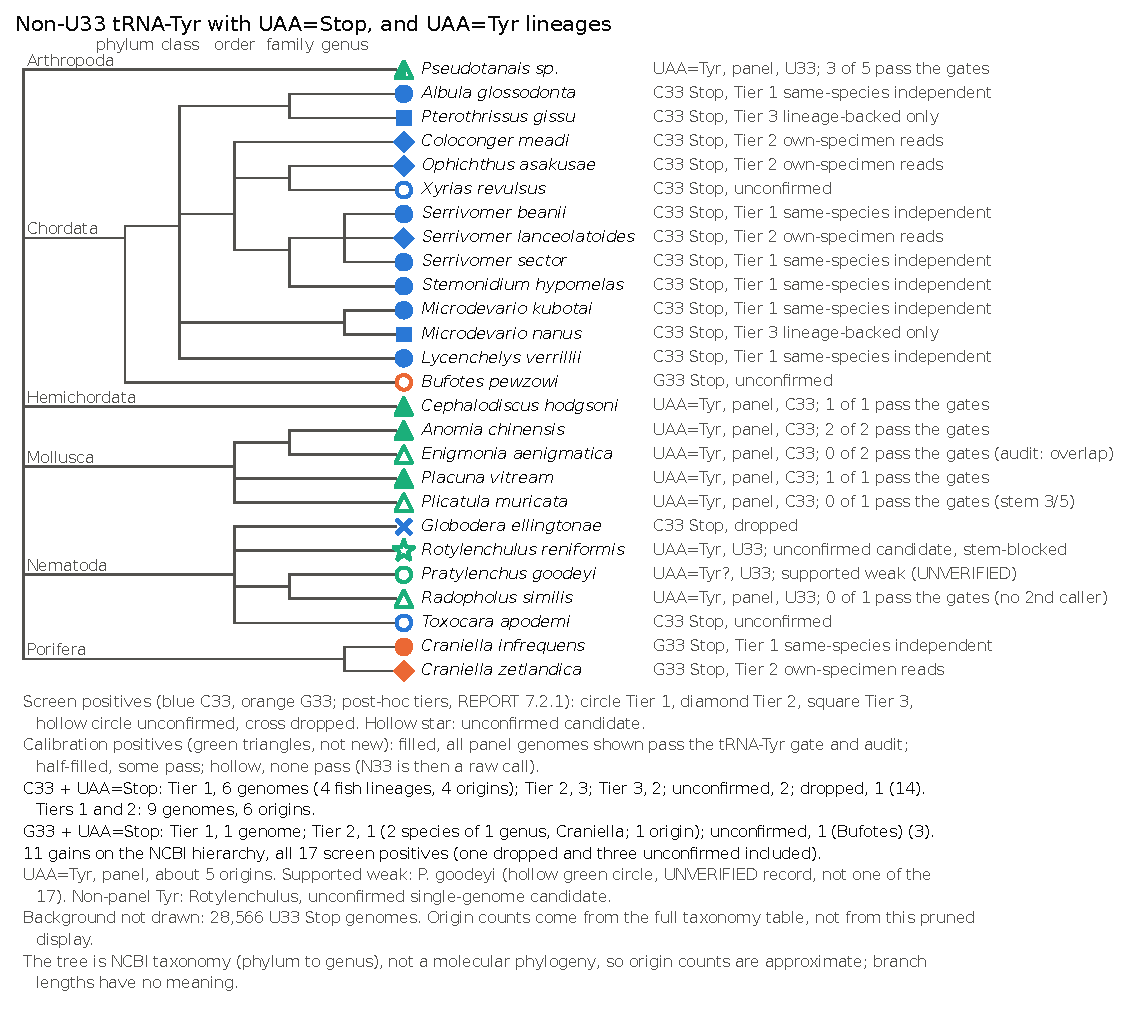
\includegraphics[width=18.2cm]{figures/fig1_tree.pdf}}
\caption{\textbf{Taxonomic distribution of non-U33 tRNA-Tyr(GUA) screen positives and calibration UAA=Tyr lineages across Metazoa.} Pruned NCBI taxonomy display of all 17 locked confirmatory UAA=Stop non-U33 screen positives (14 C33, 3 G33), with known calibration UAA=Tyr lineages, the unconfirmed single-genome candidate \textit{Rotylenchulus reniformis}, and \textit{Pratylenchus goodeyi}, a supported-weak \texttt{UNVERIFIED} record from the exploratory sweep that is not one of the 17 (hollow green circle). The background of 28,566 U33 UAA=Stop genomes is not drawn. Symbols distinguish post-hoc evidence tiers (\texttt{[P]}: Tier 1 same-species independent, Tier 2 own-specimen reads, Tier 3 lineage-backed, unconfirmed, and dropped \textit{Globodera ellingtonae}) and separate calibration positives by molecular-gate pass/fail status (including \textit{Enigmonia}, \textit{Radopholus}, and \textit{Plicatula muricata}, which fail the locked audit or gate). The annotation of 11 origins denotes minimum gains on the NCBI taxonomy hierarchy across all 17 screen positives (including the dropped hit) under a no-reversal count, rather than 11 demonstrated independent evolutionary events.}\label{fig:fig1}
\end{figure}

\begin{figure}[!htbp]
\centering
\makebox[\textwidth][c]{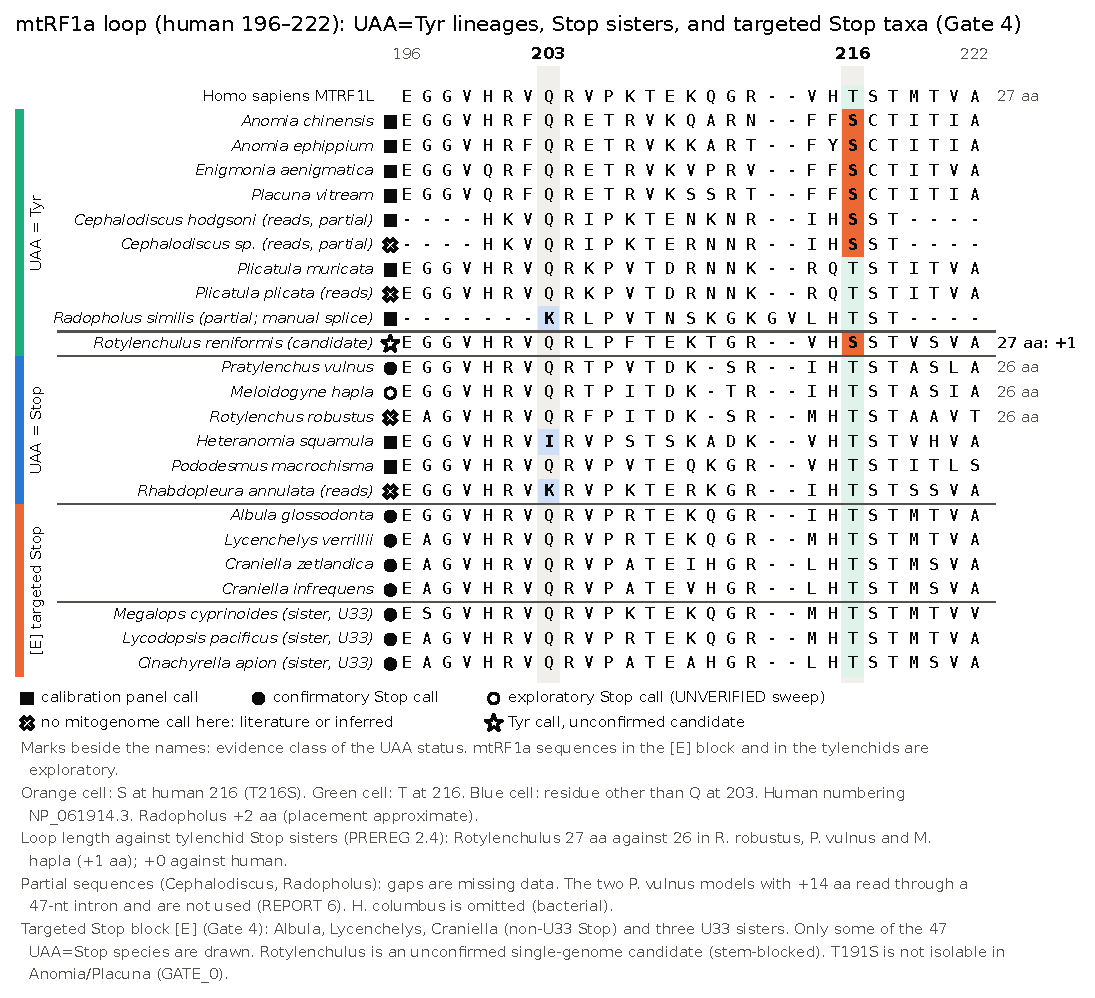
\includegraphics[width=18.2cm]{figures/fig2_mtrf1a_loop.pdf}}
\caption{\textbf{mtRF1a codon-recognition loop alignment and Q203/T216 genotypes across UAA=Tyr lineages, flagged candidates, and canonical UAA=Stop taxa.} Alignment of the mtRF1a recognition loop (human \texttt{NP\_061914.3} residues 196--222, anchored on \texttt{VPxTE} and \texttt{GRxHTS}) comparing calibration UAA=Tyr lineages (Anomiidae/Placunidae, \textit{Cephalodiscus}, Plicatulidae, \textit{Radopholus}), the exploratory unconfirmed candidate \textit{Rotylenchulus reniformis} (Q203, S216, loop $+1$ relative to 26-aa canonical tylenchid sisters \textit{P.\ vulnus}, \textit{M.\ hapla}, and \textit{R.\ robustus}, excluding two frameshifted intron-readthrough $+14$ models in \textit{P.\ vulnus}), and UAA=Stop species. Only a subset of the UAA=Stop species is drawn; 47 have both a UAA call in this study and a readable position 216, and all 47 have T216. The block labelled ``targeted Stop'' \texttt{[E]} holds the species chosen in Gate 4 for the C33 and G33 screen positives: those with nuclear data, and their U33 sisters. Status marks distinguish evidence classes, including taxa without a mitogenome UAA call in this study (\textit{Cephalodiscus} sp., \textit{Plicatula plicata}, \textit{Rotylenchus robustus}, and \textit{Rhabdopleura annulata}, whose Stop status comes from the literature on its congener) and exploratory \texttt{UNVERIFIED}-sweep Stop \textit{M.\ hapla}.}\label{fig:fig2}
\end{figure}

\begin{figure}[!htbp]
\centering
\makebox[\textwidth][c]{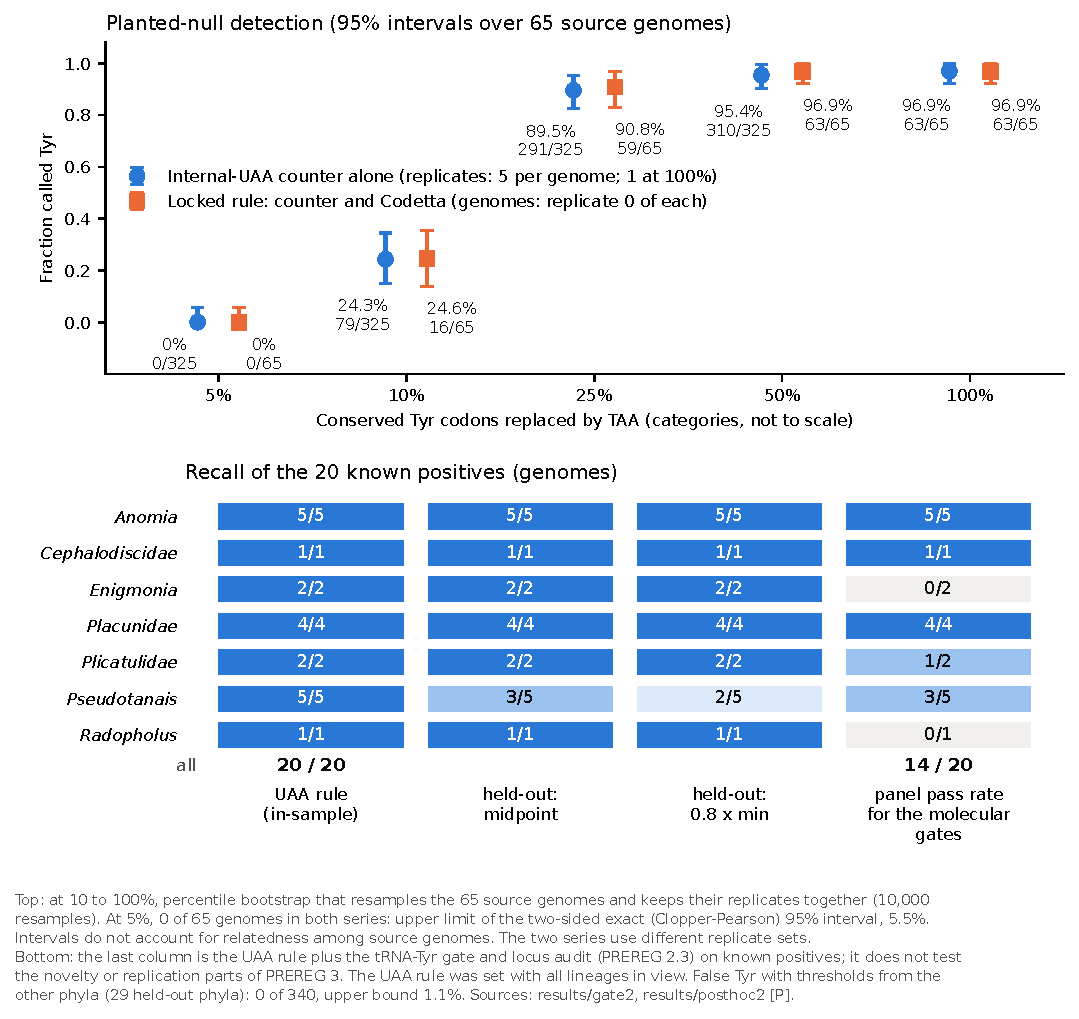
\includegraphics[width=18.2cm]{figures/fig3_sensitivity.pdf}}
\caption{\textbf{Calibration sensitivity, leave-one-lineage-out stability, and molecular-gate panel pass rate.} \textbf{Top:} planted-null recall at 5\%, 10\%, 25\%, 50\%, and 100\% of conserved Tyr codons replaced by TAA across 65 source genomes (categorical x-axis), for two series. The internal-UAA counter alone (circles; 5 replicates per genome, 1 at 100\%) called 0, 24.3, 89.5, 95.4, and 96.9\% of replicates, with genome-clustered bootstrap 95\% intervals of 15.1--34.5\%, 82.5--95.4\%, 90.2--99.4\%, and 92.3--100\% at 10--100\%. The locked rule, counter and Codetta (squares; one replicate per genome) called 0, 24.6, 90.8, 96.9, and 96.9\% of genomes, with intervals of 13.9--35.4\%, 83.1--96.9\%, 92.3--100\%, and 92.3--100\%. At 5\%, the interval is the exact two-sided binomial 95\% upper bound on 0/65 genomes (5.5\%; \texttt{[P]}). \textbf{Bottom:} leave-one-lineage-out recall of the 20 known positives and the panel pass rate for the combined molecular gates (14 of 20 known positives vs.\ 20 of 20 for the UAA rule alone; 0 for \textit{Enigmonia} and \textit{Radopholus}). Held-out phylum false positives: 0/340 (Wilson 95\% upper bound 1.1\%; \texttt{GATE\_2 A11}).}\label{fig:fig3}
\end{figure}

% --- SUPPLEMENTARY INFORMATION OUTLINE ---
\clearpage
\section*{Supplementary Information Outline}
The following companion files from the v3 archive (\texttt{commit 35bf5df}) comprise the Supplementary Information package for bioRxiv submission:
\begin{itemize}[leftmargin=1.4em, itemsep=0.25em]
\item \textbf{Supplementary Table S1:} Complete per-run read-power table (all 23 primary checks and 13 competitive body-alignment checks with exact one-sided 95\% Clopper--Pearson upper bounds; \path{results/posthoc2/read_power.tsv}, \path{read_power_check4.tsv}).
\item \textbf{Supplementary Table S2:} Conspecific specimen metadata and \textit{COX1}/mitogenome divergence audit for the five Tier 1 fish and panel \textit{A.\ vulpes} (\path{results/posthoc2/conspecific_specimen_audit.tsv}).
\item \textbf{Supplementary Table S3:} Phylum-stratified tRNA-Tyr completeness (\texttt{resolved}, \path{stem_audit_review}, \texttt{unresolved}, \texttt{wrong-locus}) across all 32,623 confirmatory genomes (\path{reports/REPORT.md} \S 4.3).
\item \textbf{Supplementary Table S4:} Species-by-species mtRF1a denominator list (47 UAA=Stop species plus excluded \texttt{MTRF1}-only and uncalled taxa; \path{results/posthoc2/mtrf1a_stop_denominator.tsv}).
\item \textbf{Supplementary Table S5:} High-copy contig search summary and non-mitochondrial contig annotations (\path{results/posthoc2/secondcopy/highcopy_summary.txt}, \path{beanii_contig.txt}, \path{contig_id_St_hypomelas.txt}).
\item \textbf{Supplementary Table S6:} Terminal stops and poly(A) junctions of the six Tier 1 fish, per gene (\path{results/posthoc2/sixfish_terminal_uaa.tsv}, \path{sixfish_terminal_genes.tsv}, \path{sixfish_polya_junctions.tsv}, \path{sixfish_polya_positions.tsv}).
\item \textbf{Supplementary Table S7:} C33 in Elopomorpha and other vertebrates (\path{results/posthoc2/elopomorpha_c33.tsv}).
\item \textbf{Supplementary Note S1:} Per-accession evidence dossiers for all 17 screen positives, \textit{R.\ reniformis}, and \textit{P.\ goodeyi} (\path{reports/dossiers/}).
\item \textbf{Supplementary Note S2:} Pre-specified \textit{R.\ reniformis} locus evaluation criteria and results (\path{results/posthoc2/roty_criteria.md}, \path{roty_eval.txt}) and \textit{Craniella} circular-mtDNA depth tables (\path{craniella_depth*.txt}).
\item \textbf{Supplementary Note S3:} Verbatim cold-review archives and item-by-item disposition tables (\path{reports/COLD_REVIEW.md}, \path{reports/COLD_REVIEW_2.md}, \path{reports/REPORT.md} \S 11 and \S 11b).
\end{itemize}

\end{document}